\documentclass{classrep}
\usepackage[utf8]{inputenc}
\usepackage[dvipsnames]{color}
\usepackage{amsmath}
\usepackage[T1]{fontenc}
\usepackage{graphicx}
\usepackage[section]{placeins}
\usepackage{listings}
\usepackage{xparse}
\usepackage{pgfplots}
\usepackage{xcolor}
\usepackage{indentfirst}

\NewDocumentCommand{\codeword}{v}{%
\texttt{\textcolor{blue}{#1}}%
}

\studycycle{Informatyka, studia niestacjonarne, I st.}
\coursesemester{VI}

\coursename{Komputerowe systemy rozpoznawania}
\courseyear{2019}

\courseteacher{dr hab. inż. Adam Niewiadomski}
\coursegroup{Niedziela, 12:00}

\author{
  \studentinfo{Konrad Jachimstal}{211807} \and
  \studentinfo{ Patryk Janicki}{211951}
}

\title{Zadanie 1: Ekstrakcja cech, miary podobieństwa, klasyfikacja}

\begin{document}
\pgfplotsset{scaled y ticks=false}
\maketitle

\section{Cel}
{Celem zadania jest zbadanie wpływu ekstrakcji cech oraz wykorzystanych miar podobieństwa w procesie klasyfikacji tekstu. 
Klasyfikacja tekstów ma zostać zrealizowania z wykorzystaniem algorytmu najbliższych sąsiadów (KNN).}

\section{Wprowadzenie}
Do wykonania tego zadania niezbędne będzie skorzystanie z uczenia maszynowego.
Klasyfikacja tekstów odbywać się będzie za pomocą algorytmu KNN. Polega ona na przypisaniu tekstu do odpowiedniej
kategorii. Odbywa się to na podstawie watrości poszczególnych wyekstrachowanych cech, które posiada każdy z tekstów.\\
Do ekstrakcji wykorzystywany jest znormalizowany zbiór słów badanego tekstu. Normalizacja ma na
celu wyeliminowanie niepożądanych słów oraz sprowadzenie odmian słów o tym samym znaczeniu do jednego (określenie rdzenia słowa).
\clearpage
\subsection[]{Wykorzystane cechy} \label{wykorzystane_cechy}
\subsubsection{Występowanie słowa kluczowego}
Na podstawie dostarczonego słowa kluczowego określamy czy to słowo występuje w dokumencie (reprezentacja binarna).
Przy użyciu tej cechy nie bierzemy pod uwagę liczności występowania tego słowa kluczowego. Cecha przyjmuje wartości $\{0; 1\}$.
\begin{equation}
    F=\left\{\begin{matrix}
                 1, & kiedy\ w = t_{i}\\
                 0, & w\ przeciwnym\ przypadku
    \end{matrix}\right.
\end{equation}
gdzie:\\
\begin{description}
    \item $w$ - dane słowo kluczowe;
    \item $t_{1}$ - kolejne słowa występujące w tekście;
\end{description}

\subsubsection{Liczba wystąpień słowa kluczowego}
Na podstawie dostarczonego słowa kluczowego określamy liczbę wystąpień tego słowa w dokumencie. Wykorzystanie tej cechy dla listy
słów kluczowych pozwala na stwierdzenie  jak licznie występuje każde słowo kluczowe w dokumencie. Chcemy sprawdzić,
czy określenie liczności słów kluczowych ma istotny wpływ na klasyfikację dokumentu.
\begin{equation}
    F=\sum_{i=0}^{n} S(w)
\end{equation}
gdzie:
\begin{equation} \label{eq:1}
    S(w)=\left\{\begin{matrix}
                    1, & kiedy\ w = t_{i}\\
                    0, & w\ przeciwnym\ przypadku
    \end{matrix}\right.
\end{equation}\\ oraz:
\begin{description}
    \item $t_{i}$ - kolejne słowa występujące w tekście;
    \item $n$ - liczba słów kluczowych;
\end{description}

\subsubsection{Suma wystąpień słów kluczowych}
Wystąpienie w dokumencie wszystkich słów kluczowych z listy ma istotny wpływ na to w jakim stopniu dany tekst
przynależy do danej etykiety. Cecha to liczba całkowita przyjmująca wartości z przedziału $<0; n>$ gdzie $n$ liczba słów w tekście.
\begin{equation}
    F=S_{1} + ... + S_{n}
\end{equation}
gdzie:\\
\begin{description}
    \item $S$ - liczba wystąpień słowa kluczowego;
\end{description}

\clearpage
\subsubsection{Gęstość występowania słów kluczowych}
Wyliczenie gęstości słów klyczowych pozwala na sprawdzenie czy cały dokument stanowi na dany temat czy jest to
jedynie wzmianka. Cecha to liczba przyjmująca wartości z zakresu $<0; 1>$.
    \begin{equation}
      F=\frac{S}{L}
    \end{equation}
gdzie:\\
\begin{description}
    \item $S$ - suma wystąpień słów kluczowych;
    \item $L$ - liczba wszystkich słów w tekście;
\end{description}

\subsubsection{Odległość słowa kluczowego od początku tekstu}
Odległość słowa kluczowego od początku tekstu wyrażona za pomocą sumy liczby wyrazów poprzedzających
dane słowo kluczowe.
Cecha przyjmuje wartości liczbowe z zakresu $<0; n>$, gdzie $n$ - liczba wyrazów poprzedzających słowo kluczowe.
\begin{equation}
    F=\sum_{0}^{n}1
\end{equation}
gdzie:\\
\begin{description}
    \item $n$ - liczba wyrazów poprzedzających dane słowo kluczowe;
\end{description}


\subsubsection{Średnia odległość słów kluczowych od początku tekstu}
Średnia odległość słów kluczowych wyrażona jako iloraz sumy odległości słów kluczowych od początku tekstu i liczby
słów kluczowych w tekście. Cecha to suma wartości liczbowych odzwierciedlających odległość danego słowa kluczowego
od początku tekstu, gdzie pojedyncze słowo odpowiada odległości równej jeden. Cecha przyjmuje wartości $<0; n>$ gdzie n
jest maksymalną średnią z sumy odległości słów kluczowych od początku tekstu.
\begin{equation}
    F=\frac{S_{1} + ... + S_{n}}{L}
\end{equation}
gdzie:\\
\begin{description}
    \item $S$ - odległość słowa kluczowego od początku tekstu;
    \item $L$ -  liczba słów kluczowych w tekście;
\end{description}

\subsubsection{Pierwsze słowo kluczowe}
Pierwsze słowo kluczowe przyjmuje wartość pierwszego napotkanego słowa kluczowego w tekście. Cecha przyjmuje wartość
tekstową odpowiadającą pierwszemu napotkanemu słowu kluczowemu.
\begin{equation}
    F= h(i)=\left\{\begin{matrix}
       w, & w = t_{i}
    \end{matrix}\right.
\end{equation}
gdzie:\\
\begin{description}
    \item $w$ - dane słowo kluczowe;
    \item $t_{i}$ - kolejne słowa występujące w tekście;
\end{description}

\subsubsection{Najczęściej występujące słowo kluczowe}
Najczęściej występujące słowo kluczowe wyrażone jako tekst odpowiadający największej liczbie wystąpień danego
słowa kluczowego w tekście. Cecha przyjmuje wartość tekstową odpowiadającą najczęściej występującemu słowu kluczowemu.
\begin{equation}
    F= w_{max_{i}(h(w_{i}), h(w_{i}))}
\end{equation}
gdzie:
\begin{equation}
    h(w)=\sum_{i=0}^{n} S(w)
\end{equation}
\begin{description}
    \item $S(w)$ - według wzoru (\ref{eq:1});
    \item $w$ - dane słowo kluczowe;
    \item $t_{i}$ - kolejne słowa występujące w tekście;
\end{description}

\subsubsection{Liczba wszystkich słów}
Określenie liczby wszystkich słów występujących w tekście. 
Cecha przyjmuje wartość $n$ równą liczbie słów w tekście.
\begin{equation}
    F=|S|
\end{equation}
gdzie:\\
\begin{description}
    \item $S$ - to zbiór słów występujących w tekście;
\end{description}

%\subsubsection{Rozproszenie słów kluczowych}
%Rozproszenie słów kluczowych wyrażone jako iloraz sumy odległości pomiędzy słowami kluczowymi i iloczyn liczby
%wszystkich słów w tekście oraz liczby słów kluczowych w tekście.
%
%Możemy podjąć próbę i założyć, że większe nagromadzenie słów kluczowych na przestrzeni całego tekstu pozwala
%stwierdzić, czy określone słowa kluczowe mają powiązanie z tematem tekstu, a nie stanowią wzmianki czy wstępu do
%tekstu. Ekstrakcja ma pozwolić na określenie rozrzutu słów kluczowych w tekście. Cecha jest określona na podstawie
%sumy odległości pomiędzy słowami kluczowymi z uwzględnieniem gęstości ich występowania. Przyjmuje wartości $[0, \infty]$.
%\begin{equation}
%    F=\frac{E_{d}}{N*N_{k}}
%\end{equation}
%gdzie:\\
%\begin{description}
%    \item $E_{d}$ - suma odległości pomiędzy słowami kluczowymi;
%    \item $N$ - liczba wszystkich słów w tekście;
%    \item $N_{k}$ - liczba słów kluczowych w tekście;
%\end{description}

%\subsubsection{Występowanie określonych podciągów}
%\dots
\subsection{Określanie istotności słów}
Podczas analizy tekstu można zauważyć, że niektóre słowa są bardziej lub mniej istotne. W związku z tym zależy nam
na eliminacji słów nieznaczących i wyodrębnieniu słów istotnych w kontekście dokumentu. Istotność słów możemy określić
na podstawie następujących algorytmów opisanych poniżej.


\subsubsection{Częstość słów (ang. Term Frequency)}
Liczba wystąpień słowa w dokumencie w stosunku do wszystkich słów pozwala nam na określenie częstotliwości występowania
określonego słowa. Zakładamy, że słowo, które występuje stosunkowo rzadko w dokumencie jest wysoce istotne. Zależność tą
można określić za pomocą wzoru:
\begin{equation}
    F=\frac{K}{W}
\end{equation}
gdzie:\\
\begin{description}
    \item $K$ - liczba wystąpień danego słowa kluczowego w dokumencie;
    \item $W$ - liczba wszystkich słów w dokumencie;
\end{description}

\subsubsection{IDF (ang. inverse document frequency)}
Możemy określić w ilu dokumentach występuje dane słowo. Jeśli słowo występuje w małej liczbie dokumentów lub tylko w
jednym, można stwierdzić, że to słowo jest ściśle powiązane z treścią tych dokumentów. Zależność tą można określić za
pomocą wzoru:
\begin{equation}
    F=log \frac{W}{D}
\end{equation}
gdzie:\\
\begin{description}
    \item $W$ - liczba wszystkich dokumentów;
    \item $D$ - liczba dokumentów w których wystąpiło słowo kluczowe;
\end{description}

\subsubsection{TF-IDF}
Jest to połączenie częstości słów występujących w dokumencie zestawione z stosunkiem wytępowania tego słowa we wszystkich
dokumentach. Połączenie tych cech pozwala na uzależnienie istotności słowa nie tylko od dokumentu w którym występuje,
ale również od występowania w całym zbiorze dokumentów. Zależność tą można określić za pomocą wzoru:
\begin{equation}
    F={TF}\cdot{IDF}
\end{equation}
gdzie:\\
\begin{description}
    \item $TF$ - częstość słów w danym dokumencie;
    \item $IDF$ - częstość występowania na tle innych dokuemntów;
\end{description}

\subsubsection{Generowanie stop listy}
Tworzenie stop listy opieramy na algorytmie IDF. Słowo które ma najmniejszą wartość IDF występuje najczęściej. Czyli jest
nieistotne. Dodajemy do stoplisty jeśli dana wartość będzie poniżej określonego progu.

\subsubsection{Nauka słów kluczowych}
Do nauki słów kluczowych wykorzystujemy algorytm TF-IDF, za pomocą którego określamy istotność
danego słowa. Kiedy dla danego słowa wartość ta jest większą od założonej, uznajemy to słowo za istotne tym samym dopisując je do
listy słów kluczowych. Słowa kluczowe mogą zostać również określone odgórnie. Ponadto mogą być również wygenerowane
za pomocą algorytmu TF.
Wtedy niezależnie od liczności danej etykiety
zostanie wybrana tylko określona liczba słów.

\subsection{Metryki - miara odległości} \label{wykorzystane_metryki}
Wykorzystane metryki służa do określenia odległości pomiędzy elementami tego samego zbioru w naszym przypadku tym
zbiorem będzie zbiór artykułów. Do obliczenia odległości pomiędzy dwoma artykułami na potrzeby algorytmu KNN zostały
wykorzystane metryki opisane poniżej.

\subsubsection{Metryka Euklidesowa}
Odległość Euklidesowa jest to odległość między dwoma wektorami określona jako pierwiastek kwadratowy sumy różnic między
wartościami podniesionymi do kwadratu, wyrażona wzorem:
\begin{equation}
    d(x,y)=\sqrt{\sum_{i=1}^{n}((x_{i}-y_{i})^{2})}
\end{equation}
gdzie:\\
\begin{description}
    \item $d$ - miara odległości;
    \item $x$, $y$ - wartości cech;
\end{description}

\subsubsection{Metryka Czebyszewa}
Odległość Czebyszewa jest to różnica pomiędzy znormalizowanymi cechami wartości obiektów, określona wzorem:
\begin{equation}
    d(x,y)=max_{i}|x_{i}-y_{i}|
\end{equation}
gdzie:\\
\begin{description}
    \item $d$ - miara odległości;
    \item $x$, $y$ - wartości cech obiektów;
\end{description}

\subsubsection{Metryka Manhattana}
Metryka Manhattana jest metryką podobną do metryki euklidesowej z tą różnicą, że odległość wyliczana jest
z bezwzględnych różnic pomiędzy wektorami. Odległość tę wyraża się wzorem:
\begin{equation}
    d(x,y)=\sum_{i=1}^{n} |x_{i}-y_{i}|
\end{equation}
gdzie:\\
\begin{description}
    \item $d$ - miara odległości;
    \item $x$, $y$ - wartości cech obiektów;
\end{description}

\subsection{Miary podobieństwa tekstów}
Miara podobieństwa tesktów to miara mówiąca o tym w jakim stopniu dany tekst $A$ jest podobny do tekstu $B$.

\subsubsection{Metoda n-gramów} \label{n_gram}
Metoda n-gramów określa w jakim stopniu łańcuch znaków $x$ jest podobny do łańcucha znaków $y$, na podstawie podciągów.
\begin{equation}
    sim_{n}(x,y)=\frac{1}{N-n+1}\sum_{i=1}^{N-n+1}h(i)
\end{equation}
gdzie:\\
\begin{description}
    \item $h(i)$ - przyjmuje 1 jeżeli dany podciąg występuje w łancuchu znaków $y$, w przeciwnym wypadku przyjmuje wartość 0;
    \item $N$ - liczba liter w słowie;
    \item $n$ - długość n-grama;
    \item $N-n+1$ - ilość n-elementowych podciągów w łańcuchu znaków;
\end{description}

\subsubsection{Uogólniona miara n-gramów}
Uogólniona miara n-gramów sprawdza podobieństwo słów w oparciu o podciągi o określonej długości. Wyrażona jest wzorem:

\begin{equation}
    u_{N}(x, y)=\frac{2}{N^{2}+N}\sum_{i=1}^{N(x)}\sum_{j=1}^{N(x-i+1)}h(i,j)
\end{equation}
gdzie:\\
\begin{description}
    \item $h(i,j)$ przyjmuje wartość 1 jeżeli dany podciąg ze słowa $x$ znajduje się w słowie $y$;
    \item $N(x),N(y)$ - ilość liter w słowach $x, y$, $N=max{N(x),N(y)}$;
    \item $\frac{N^{2}+N}{2}$ - ilość możliwych podciągów 1-elementowych do N-elementowych w słowie o długości $N$;
\end{description}

\subsubsection{Algorytm KMP (Knutha-Morrisa-Pratta)}
Algorytm KMP wyszukuje podany wzorzec $x$ w tekście $y$, jeżeli podany wzorzec zostaje znaleziony zwracana jest jego
pozycja w tekście.

\subsection{Normalizacja (Zero-Mean)}
Normalizacji poddawany jest każdy wektor cech. Działanie to eliminuje sutyację, w której wartość pewnej
cechy może zdominować cały wektor cech.

    \begin{equation}
        V'=\frac{V-\bar{U}}{\sigma}
    \end{equation}
    gdzie:\\
    \begin{description}
        \item $V'$ - znormalizowana wartość cechy;
        \item $V$ - wartość cechy;
        \item $\bar{U}$ - średnia z wektora cech;
        \item $\sigma$ - odchylenie standardowe z wektora cech;
    \end{description}

\subsection{Określanie poprawności klasyfikacji} \label{poprawnosc_klasyfikacji}
Poprawność sklasyfikowanych danych określa w jakim stopniu dokumenty zostały poprawnie przyporządkowane etykietom.
Wartość poprawności będzie oscylować w przedziale $<0;1>$. Kiedy wartość będzie będzie zbliżać się do jedynki będzie
to oznaczać, że większość dokumentów została sklasyfikowana poprawnie.

\begin{equation}
    F=\frac{P}{W}
\end{equation}
gdzie:\\
\begin{description}
    \item $P$ - liczba poprawnie sklasyfikowanych dokumentów;
    \item $W$ - liczba wszystkich klasyfikacji;
\end{description}

%{\color{blue}
%We wprowadzeniu należy zaprezentować całą teorię potrzebną do realizacji
%zadania (przy czym należy tu ograniczyć się wyłącznie do tego, co było
%wykorzystane) tak aby osoba, która nigdy wcześniej nie zetknęła się z tą
%tematyką, potrafiła zrozumieć dalszy opis. Część ta powinna wprowadzać
%wszystkie wykorzystywane wzory, oznaczenia itp., do których należy się
%odwoływać w dalszej części niniejszgo sprawozdania. Zamieszczony tu własny
%opis teorii (a nie skopiowany!) należy poprzeć odwołaniami bibliograficznymi
%do literatury zamieszczonej na końcu. }

\section{Opis implementacji}
\subsection{Struktura projektu}
Projekt został zrealizowany w języku Java. W celu uporządkowania projektu utworzona została następująca struktura:
\begin{itemize}
    \item \textbf{data\_models} - obsługa przygotowania obiektów do klasyfikacji
    \item \textbf{features} - ekstraktory oraz implementacja cech
    \item \textbf{helpers} - metody pomocnicze
    \item \textbf{metrics} - klasy realizujące miary odległości
    \item \textbf{similarity} - klasy realizujące miary podobieństwa tekstu
    \item \textbf{utils} - narzędzia do manipulacji danymi (stemizacja, słowa kluczowe, stoplista, zapis/odczyt, ...)
\end{itemize}

\subsection{Najważniejsze składowe}
Aby zachować niezależność od obiektów, które podlegają klasyfikacji, utworzono interfejs \codeword{IClassificationObject}.
Interfejs gwarantuje, aby klasyfikowany obiekt posiadał metody udostępniające dane wymagane do klasyfikacji. Dodatkowo 
stworzono interfejsy \codeword{IMetric} oraz \codeword{ISimilarity}, których implementacja pozwala na dostarczenie
nowych metryk lub miar podobieństwa. Klasa \codeword{Extraction} zawiera ekstraktory cech, które tworzą mapę obiektów 
\codeword{IFeature} wewnątrz klasy. Każde użycie ekstraktora powoduje dodanie cech do mapy, która staje się wektorem 
cech danego obiektu. Klasa \codeword{Classification} dokonuje podziału dostarczonych obiektów na dwie grupy zgodnie
z ustalonym współczynnikiem podziału oraz odpowiada za realizację wszystkich zadań - wywołuje metody realizujące
stemizację, normalizację, ekstrakcję, generowanie słów kluczowych i ostatecznie klasyfikację.
% Z powyższych pakietów możemy wyszczególnić najważniejsze klasy ze względu na tematykę projektu. Podstawowym pakietem
% jest pakiet $data\_model$, w którym to wczytywane są z pliku artykuły a następnie dzielone na poszczególne klasy "Article".
% Klasa "Extraction" zawiera w sobie wszystkie wykorzystane w programie cechy z podziałem każdej cechy jako jedną metodę.
% Daje to możliwość skorzystania jedynie z cech, które nas interesują. W pakiecie "metrics" zostały zaimplementowane metody
% liczenia odległości pomiędzy wektorami cech na podstawie interfejsu "IMetric", w którym to zadeklarowana została
% metoda "compare" służąca do porównywania wektorów cech. Pakiet "similarity" odpowiada za liczenie odległości w
% przpadkach kiedy cecha jest słowem. Klasa "TermFrequency" wykorzystywana jest podczas generowania słów kluczowych oraz stop listy.
% Wszystkie klasy wykorzystane zostają w klasie "Classification", dokounuje się tam wszystkich operacji począwszy od podziału
% tekstów na dwa zbiory po klasyfikację tekstu do odpowiedniej etykiety.

\begin{figure}[h!]
    \centering
    \makebox[\textwidth][c]{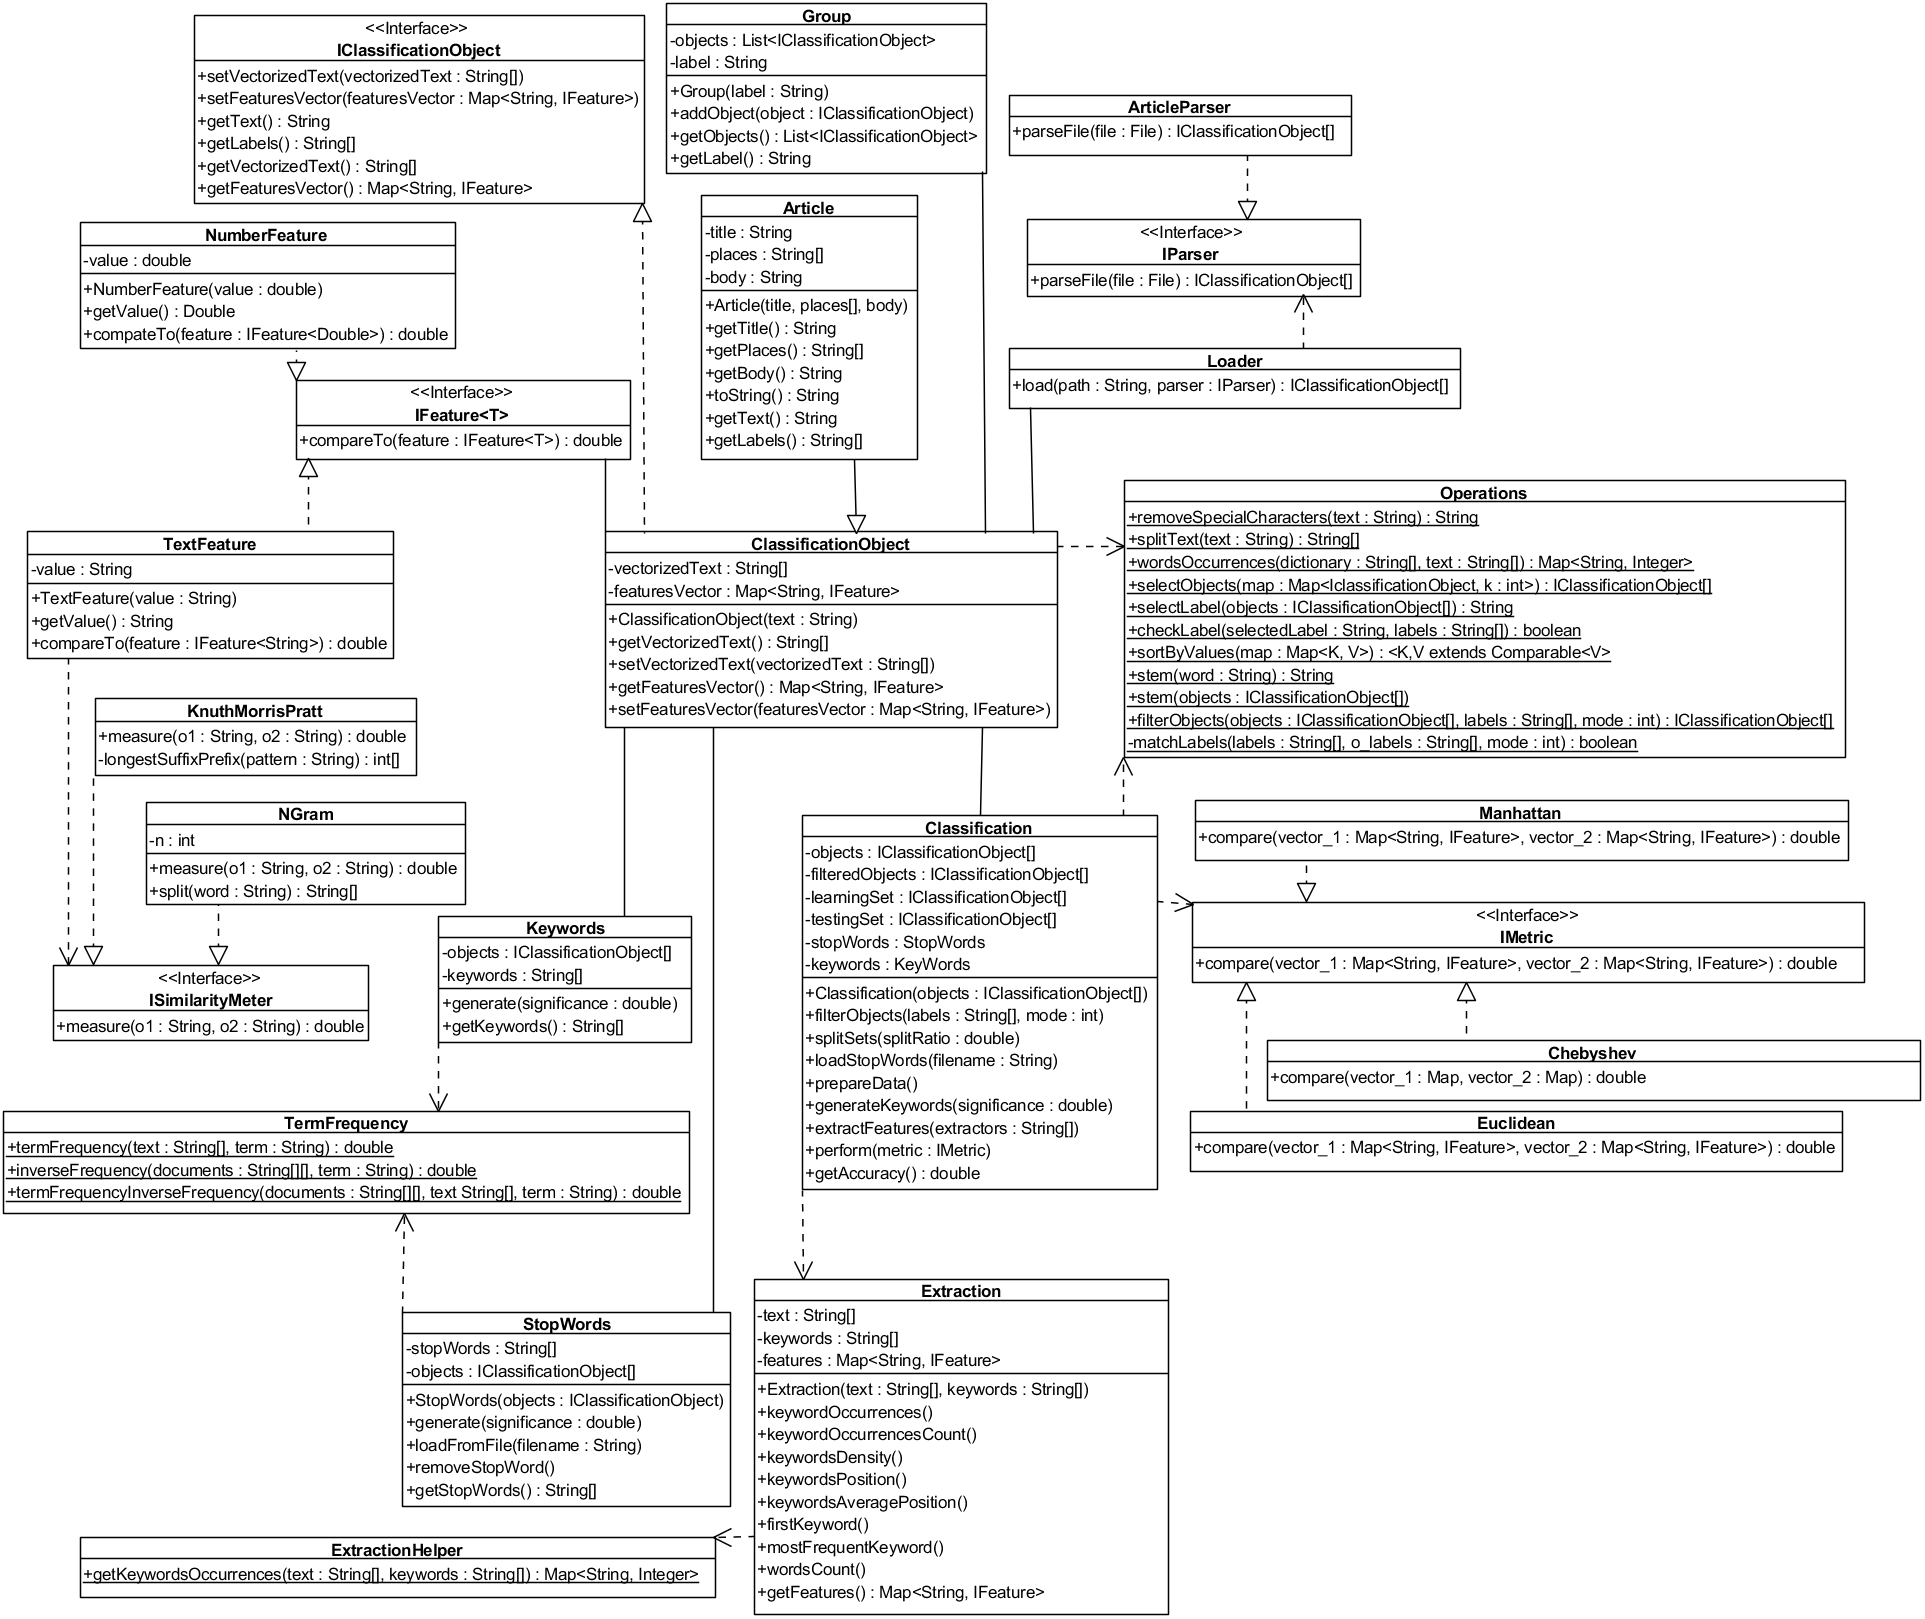
\includegraphics[width=1.3\textwidth]{uml.png}}%
    \caption{Diagram klas}
    \label{fig:uml}
\end{figure}

%{\color{blue}
%Należy tu zamieścić krótki i zwięzły opis zaprojektowanych klas oraz powiązań
%między nimi. Powinien się tu również znaleźć diagram UML  (diagram klas)
%prezentujący najistotniejsze elementy stworzonej aplikacji. Należy także
%podać, w jakim języku programowania została stworzona aplikacja. }
\section{Materiały i metody} \label{mat}
Klasyfikacja tekstów dotycząca kategorii $PLACES$ została przeprowadzna na zbiorze tekstów Reutersa, za
pomocą wszystkich zaimplmentowanych ekstraktorów cech \ref{wykorzystane_cechy}. Badania zostały
przeprowadzone dla wszystkich trzech metryk opisanych w punkcie \ref{wykorzystane_metryki}. Wartości
parametru $k$ w algorytmie klasyfikującym K najbliższych sąsiadów zostały dobrane tak aby wykazać jego
wpływ na klasyfikację. Parametr ten przyjmuje wartości ze zbioru \{2, 5, 10, 15, 20\}. Zbiór tekstów
został podzielony odpowiednio $60\%$ jako dane treningowe oraz $40\%$ jako dane testowe. Jako stop listę
wykorzystano gotowy zbiór\footnotemark[1] słów nieznaczących dla języka angielskiego.
\footnotetext[1]{https://gist.github.com/sebleier/554280}
Słowa kluczowe zostały wygenerowane na podstawie algorytmu częstości słów (TF-IDF). Podczas generowania
słów kluczowych została przyjęta wartość $0.75$ (TF-IDF) powyżej której słowo traktowane jest jako istotne i
tym samym trafia na listę słów kluczowych. Miara odległości pomiędzy wekstrachowanymi wektorami cech zawierającymi słowa
została zrealizowana za pomocą metody N-Gramów opisanej w punkcie \ref{n_gram} z parametrem $N=3$.

\\ Aby zbadać poprawność klasyfikacji posłużyliśmy się parameterm zgodności, którego wartość wskazuje
jaki procent tekstów został sklasyfikowany poprawnie (opisany w punkcie \ref{poprawnosc_klasyfikacji}).

\\Podczas klasyfikowania kategorii $TOPICS$ przyjęto etykiety: ship, tea, oraz silver.
Zbiór podzielono równo po $50\%$ dla zbioru uczącego jak i dla zbioru testowego. Stop listę wczytano z pliku
jak w poprzednim badaniu jednak współczynnik generowania słów kluczowych przyjął wartość $0,1$. Badanie
wykonano dla takich samych parametrów $k$ jak poprzednio dla lepszego porównania wyników. Porównanie odbyło
się w oparciu o te same metryki liczenia odległości pomiędzy wektorami cech dokumentów jak i tę samą metodę
obliczania odległości między cechami o wartości tekstowej.

\\Badanie ekstraktora słów kluczowych TF. Klasyfikację kategorii $TOPICS$ powtórzono zmieniając jedynie
metodę generowania słów kluczowych algorytmu TF-IDF na TF z liczbą słów równą $15$ dla każdej etykiety.

\\Własny zbiór tekstów zawierał sześć etykiet: siliconvalley, drwho, twinpeaks, got, friends, simpsons
oraz składał się ze 120 obietków. Badań dokonano na wszystkich etykietach. Zbiór podzielono
w stosunku $60:40$. Jako stop listę wykrzystano
gotowy zbiór słów nieznaczączych wymieniony powyżej. Słowa kluczowe zostały wygenerowane za pomocą
algorytmu TF-IDF ze współczynnikiem $0,7$. Jako miarę podobieństwa słów wybrano metodę Knutta-Morria-Pratta.
Klasyfikacji dokonano dla każdej z wcześniej przyjętych wartości $k$ oraz dla każdej z metryk. Oraz dla
wszystkich wcześniej przedstawionych cech.

\\Badanie dotyczące optymalnego podziału zbioru rozpoczęto od podziału $90\%$ tekstów jako zbiór uczący
$10\%$ jako testowy, kolejno do wartości $10\%$ zbiór uczący oraz $90\%$ zbiór testowy. Skorzystano z
etykiet: hongkong, sweeden, philipines. Etykiety dobrano tak aby ich liczebność była zbliżona.
Stop listę wczytano z pliku jak w poprzednich badaniach. Słowa kluczowe generowano ze współczynnikiem
TF-IDF wynoszącym $0,2$. Generowania słów kluczowych dokonywano przy każdej zmianie podziału zbioru
ze względu na zmianę liczebności zbioru uczącego. Wykorzystano wszystkie dostępne ekstraktory cech.
W badaniu parametr $k$ był
stały i wynosił $20$. Jako metrykę przyjęto metrykę Euklidesową. Liczebność zbioru na którym
przeprowadzono badanie wynosiła 206 elementów.

\\Podczas badania jak miara podobieństwa słów wpływa na poprawność klasyfikacji wykorzystano ustawienia
programu takie jak te wykorzystane podczas badania podziału zbioru. Zmianie uległa jedynie miara podobieństwa słów.
Zbiór uczący zawiarał $60\%$ wszystkich tekstów.

\\Badanie wpływu danych cech na poprawność klasyfikacji oraz czas jej trwania przeprowadzono na
etykietach: $canada$, $uk$, $west-germany$. Parametr $k$ z wartością 20, natomiast jako miarę odległości
przyjęto metrykę Euklidesową. Zbiór podzielono w stosunku $60:40$. Słowa kluczowe zostały wygenerowane
z parametrem TF-IDF równym $0,4$. Stop listę wczytano z pliku.

\\Wpływ miary podobieństwa słów w metodzie N-Gramów zbadano dla wartości $N$ równych kolejno ${1,2,3,4,5,6,7}$.
Do badania wybrano tylko cechy: najczęściej występujące słowo kluczowe oraz pierwsze słowo kluczowe, tak
aby inne cechy nie wpływały na wynik badania. Pozostałe ustawienia programu zostały ustawione tak jak podczas badania wpływu danych cech na
poprawność klasyfikacji.




%{\color{blue}
%W tym miejscu należy opisać, jak przeprowadzone zostały wszystkie badania,
%których wyniki i dyskusja zamieszczane są w dalszych sekcjach. Opis ten
%powinien być na tyle dokładny, aby osoba czytająca go potrafiła wszystkie
%przeprowadzone badania samodzielnie powtórzyć w celu zweryfikowania ich
%poprawności (a zatem m.in. należy zamieścić tu opis architektury sieci,
%wartości współczynników użytych w kolejnych eksperymentach, sposób
%inicjalizacji wag, metodę uczenia itp. oraz informacje o danych, na których
%prowadzone były badania). Przy opisie należy odwoływać się i stosować do
%opisanych w sekcji drugiej wzorów i oznaczeń, a także w jasny sposób opisać
%cel konkretnego testu. Najlepiej byłoby wyraźnie wyszczególnić (ponumerować)
%poszczególne eksperymenty tak, aby łatwo było się do nich odwoływać dalej.}

\section{Wyniki}
Wyniki zostały podzielone na sekcje, każda z sekcji przedstawia wyniki klasyfikacji tekstu
dla danego badania.
\subsection{Liczebności poszczególnych badanych zbiorów}
\subsubsection{Liczebność zbioru dla kategorii $PLACES$}

\begin{figure}[h!]
    \begin{center}
        \begin{tikzpicture}
            \begin{axis}[
            x tick label style={
            /pgf/number format/10000 sep=},
            ylabel=Ilość etykiety,
            xticklabels={,,,,,},
            enlargelimits=0.2,
            legend style={at={(0.5,-0.10)},
            anchor=north,legend columns=-1},
            ybar interval=0.7,
            ]
                \addplot
                coordinates {
                (1,10682)(0,0)(0,0)(0,0)(0,0)(0,0)
                };

                \addplot
                coordinates {
                (1,829)(0,0)(0,0)(0,0)(0,0)(0,0)
                };

                \addplot
                coordinates {
                (1,485)(0,0)(0,0)(0,0)(0,0)(0,0)
                };

                \addplot
                coordinates {
                (1,914)(0,0)(0,0)(0,0)(0,0)(0,0)
                };

                \addplot
                coordinates {
                (1,271)(0,0)(0,0)(0,0)(0,0)(0,0)
                };

                \addplot
                coordinates {
                (1,325)(0,0)(0,0)(0,0)(0,0)(0,0)
                };

                \legend{USA, Canada, Japan, UK, France, West-Germany}
            \end{axis}



        \end{tikzpicture}
    \end{center}
    \caption{Liczebność poszczególnych etykiet dla kategorii $PLACES$.}
    \label{licz_places}
\end{figure}
\FloatBarrier
\subsubsection{Liczebność zbioru dla kategorii $TOPICS$}

\begin{figure}[h!]
    \begin{center}
        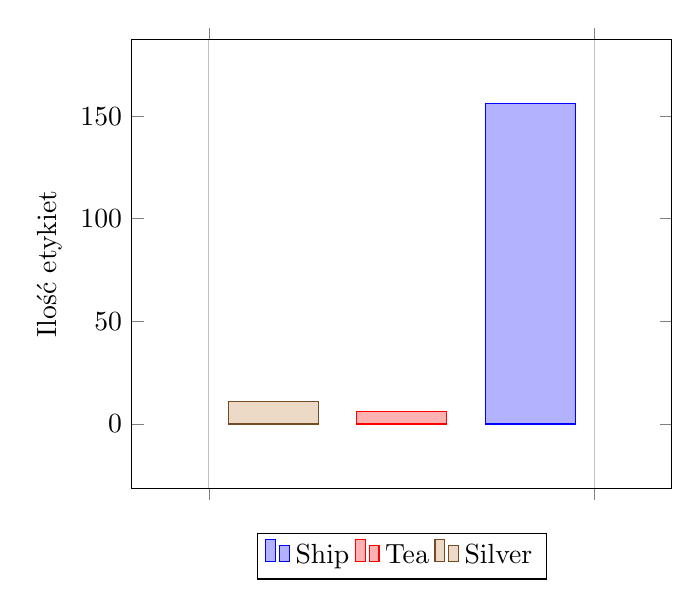
\begin{tikzpicture}
            \begin{axis}[
            x tick label style={
            /pgf/number format/1000 sep=},
            ylabel=Ilość etykiet,
            xticklabels={,,},
            enlargelimits=0.2,
            legend style={at={(0.5,-0.10)},
            anchor=north,legend columns=-1},
            ybar interval=0.7,
            ]
                \addplot
                coordinates {
                (1,156)(0,0)(0,0)
                };
                \addplot
                coordinates {
                (1,6)(0,0)(0,0)
                };
                \addplot
                coordinates {
                (1,11)(0,0)(0,0)
                };
                \legend{Ship, Tea, Silver}

            \end{axis}

        \end{tikzpicture}
    \end{center}
    \caption{Liczebność poszczególnych etykiet dla kategorii $TOPICS$.}
    \label{licz_topics}
\end{figure}

\FloatBarrier
\subsubsection{Liczebność własnego zbioru}

\begin{figure}[h!]
    \begin{center}
        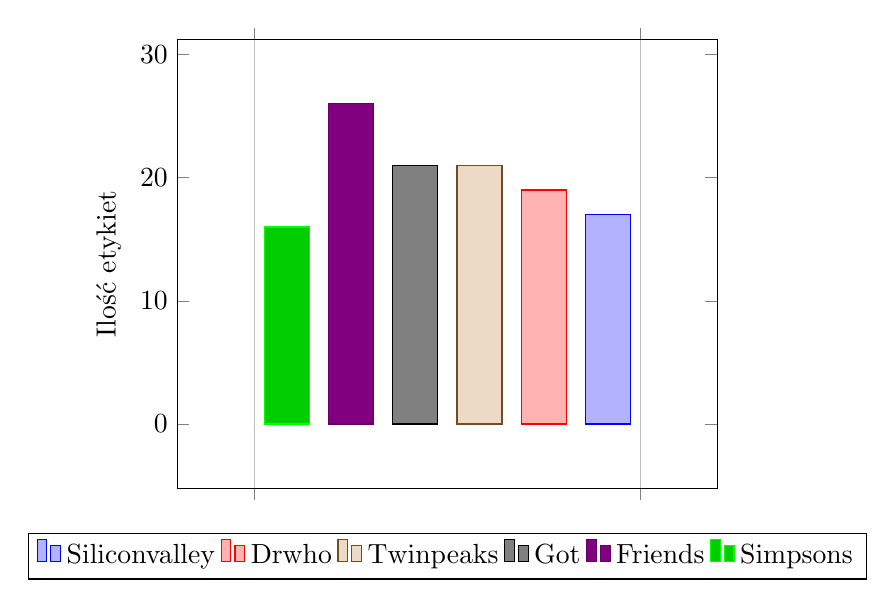
\begin{tikzpicture}
            \begin{axis}[
            x tick label style={
            /pgf/number format/1000 sep=},
            ylabel=Ilość etykiet,
            xticklabels={,,},
            enlargelimits=0.2,
            legend style={at={(0.5,-0.10)},
            anchor=north,legend columns=-1},
            ybar interval=0.7,
            ]
                \addplot
                coordinates {
                (1,17)(0,0)(0,0)
                };
                \addplot
                coordinates {
                (1,19)(0,0)(0,0)
                };
                \addplot
                coordinates {
                (1,21)(0,0)(0,0)
                };
                \addplot
                coordinates {
                (1,21)(0,0)(0,0)
                };
                \addplot
                coordinates {
                (1,26)(0,0)(0,0)
                };
                \addplot
                coordinates {
                (1,16)(0,0)(0,0)
                };
                \legend{Siliconvalley, Drwho, Twinpeaks, Got, Friends, Simpsons}

            \end{axis}

        \end{tikzpicture}
    \end{center}
    \caption{Liczebność poszczególnych etykiet dla własnego zbioru tekstów.}
    \label{licz_wlasny}
\end{figure}


\FloatBarrier
\subsection{Wyniki klasyfikacji dla kategorii $PLACES$}
Klasyfikację przeprowadzono z wykorzystaniem każdej z wcześniej wypisanych metod ekctrakcji cech. Wektor
klasyfikacji składa się z wartości tekstowych jak i liczbowych. Wyniki klasyfikacji przedstawiono poniżej
na wykresach.


\begin{figure}[h!]
    \begin{center}
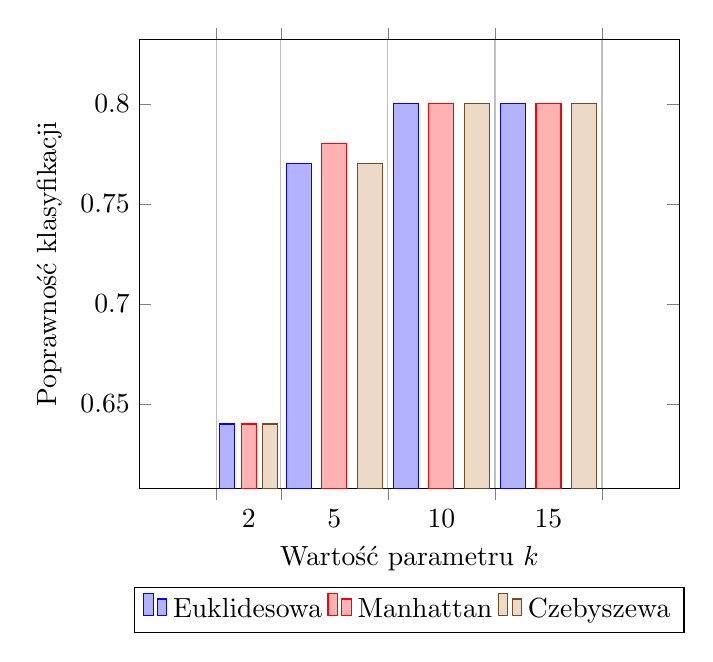
\begin{tikzpicture}
    \begin{axis}[
    x tick label style={
    /pgf/number format/1000 sep=},
    ylabel=Poprawność klasyfikacji,
    xlabel=Wartość parametru $k$,
    enlargelimits=0.2,
    legend style={at={(0.5,-0.22)},
    anchor=north,legend columns=-1},
    ybar interval=0.7,
    ]
        \addplot
        coordinates {
        (2,0.64)(5,0.77)(10,0.8)(15,0.8)(20,0.8)
        };

        \addplot
        coordinates {
        (2,0.64)(5,0.78)(10,0.8)(15,0.8)(20,0.8)
        };

        \addplot
        coordinates {
        (2,0.64)(5,0.77)(10,0.8)(15,0.8)(20,0.8)
        };

        \legend{Euklidesowa, Manhattan, Czebyszewa}
    \end{axis}

\end{tikzpicture}
\end{center}
\caption{Poprawność klasyfikacji dla wybranych wartości parametru $k$ i zawartych metryk dla kategorii
$PLACES$.}
\label{1_places}
\end{figure}

\begin{figure}[h!]
    \begin{center}
        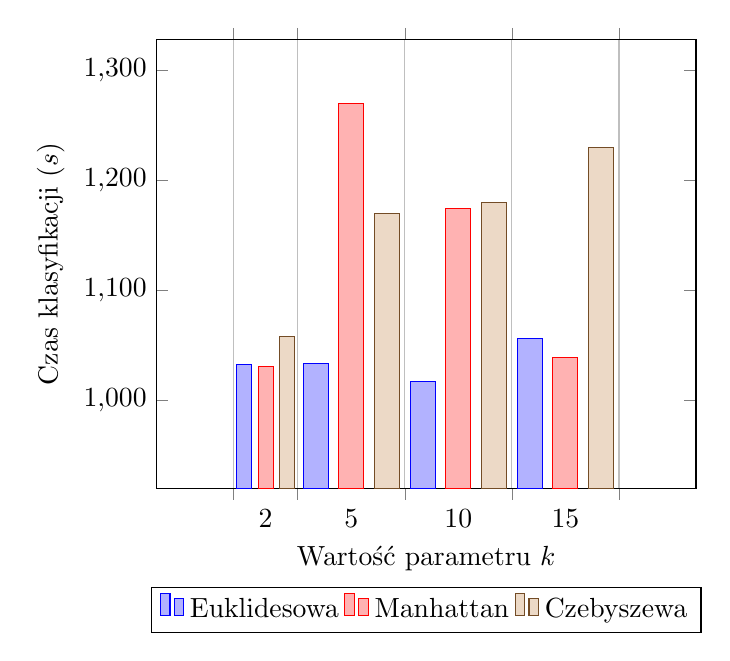
\begin{tikzpicture}
            \begin{axis}[
            x tick label style={
            /pgf/number format/1000 sep=},
            ylabel=Czas klasyfikacji ($s$),
            xlabel=Wartość parametru $k$,
            enlargelimits=0.2,
            legend style={at={(0.5,-0.22)},
            anchor=north,legend columns=-1},
            ybar interval=0.7,
            ]
                \addplot
                coordinates {
                (2,1033.047)(5,1033.665)(10,1017.195)(15,1056.296)(20,1072.138)
                };

                \addplot
                coordinates {
                (2,1030.663)(5,1269.484)(10,1174.352)(15,1039.059)(20,1089.03)
                };

                \addplot
                coordinates {
                (2,1058.355)(5,1169.824)(10,1180.133)(15,1229.68)(20,978.71)
                };

                \legend{Euklidesowa, Manhattan, Czebyszewa}
            \end{axis}

        \end{tikzpicture}
    \end{center}
    \caption{Czas klasyfikacji dla wybranych wartości parametru $k$ i zawartych metryk dla kategorii
    $PLACES$.}
    \label{1_places_time}
\end{figure}

\begin{figure}[h!]
    \begin{center}
        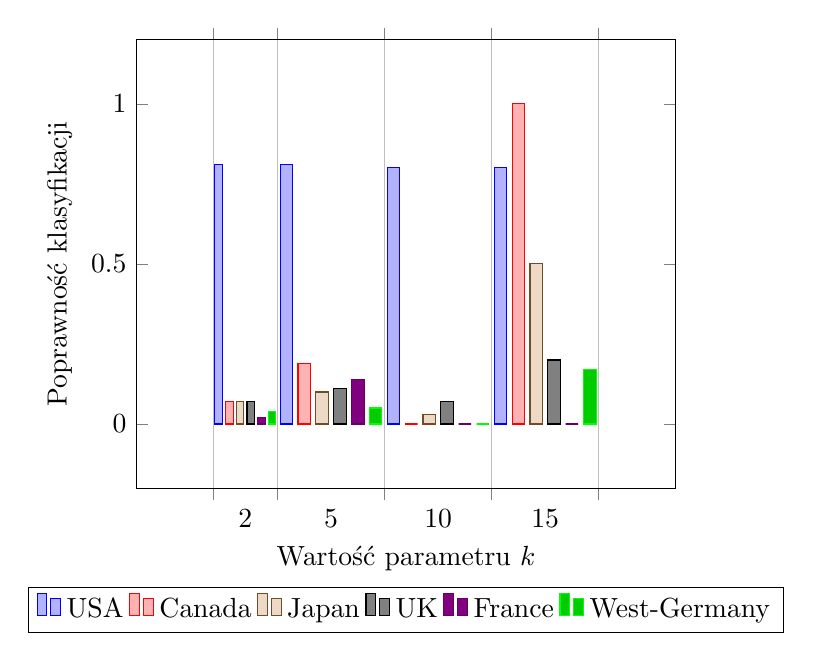
\begin{tikzpicture}
            \begin{axis}[
            x tick label style={
            /pgf/number format/1000 sep=},
            ylabel=Poprawność klasyfikacji,
            xlabel=Wartość parametru $k$,
            enlargelimits=0.2,
            legend style={at={(0.5,-0.22)},
            anchor=north,legend columns=-1},
            ybar interval=0.7,
            ]
                \addplot
                coordinates {
                (2,0.81)(5,0.81)(10,0.80)(15,0.80)(20,0.80)
                };

                \addplot
                coordinates {
                (2,0.07)(5,0.19)(10,0)(15,1)(20,0)
                };

                \addplot
                coordinates {
                (2,0.07)(5,0.10)(10,0.03)(15,0.5)(20,0)
                };

                \addplot
                coordinates {
                (2,0.07)(5,0.11)(10,0.07)(15,0.20)(20,0)
                };

                \addplot
                coordinates {
                (2,0.02)(5,0.14)(10,0)(15,0)(20,0)
                };

                \addplot
                coordinates {
                (2,0.04)(5,0.05)(10,0)(15,0.17)(20,0)
                };

                \legend{USA, Canada, Japan, UK, France, West-Germany}
            \end{axis}

        \end{tikzpicture}
    \end{center}
    \caption{Poprawność klasyfikacji etykiety dla wybranych wartości parametru
    $k$ dla kategorii $PLACES$ z użyciem metryki Euklidesowej.}
    \label{1_places_label_eucli}
\end{figure}

\begin{figure}[h!]
    \begin{center}
        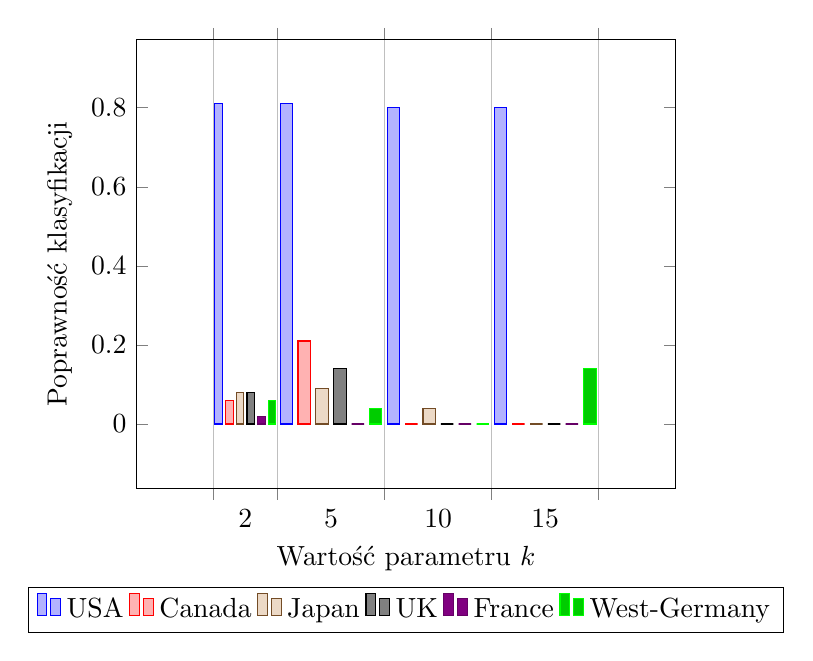
\begin{tikzpicture}
            \begin{axis}[
            x tick label style={
            /pgf/number format/1000 sep=},
            ylabel=Poprawność klasyfikacji,
            xlabel=Wartość parametru $k$,
            enlargelimits=0.2,
            legend style={at={(0.5,-0.22)},
            anchor=north,legend columns=-1},
            ybar interval=0.7,
            ]
                \addplot
                coordinates {
                (2,0.81)(5,0.81)(10,0.80)(15,0.80)(20,0.80)
                };

                \addplot
                coordinates {
                (2,0.06)(5,0.21)(10,0)(15,0)(20,0)
                };

                \addplot
                coordinates {
                (2,0.08)(5,0.09)(10,0.04)(15,0)(20,0)
                };

                \addplot
                coordinates {
                (2,0.08)(5,0.14)(10,0)(15,0)(20,0)
                };

                \addplot
                coordinates {
                (2,0.02)(5,0)(10,0)(15,0)(20,0)
                };

                \addplot
                coordinates {
                (2,0.06)(5,0.04)(10,0)(15,0.14)(20,0.11)
                };

                \legend{USA, Canada, Japan, UK, France, West-Germany}
            \end{axis}

        \end{tikzpicture}
    \end{center}
    \caption{Poprawność klasyfikacji etykiety dla wybranych wartości parametru
    $k$ dla kategorii $PLACES$ z użyciem metryki Manhattan.}
    \label{1_places_label_man}
\end{figure}

\begin{figure}[h!]
    \begin{center}
        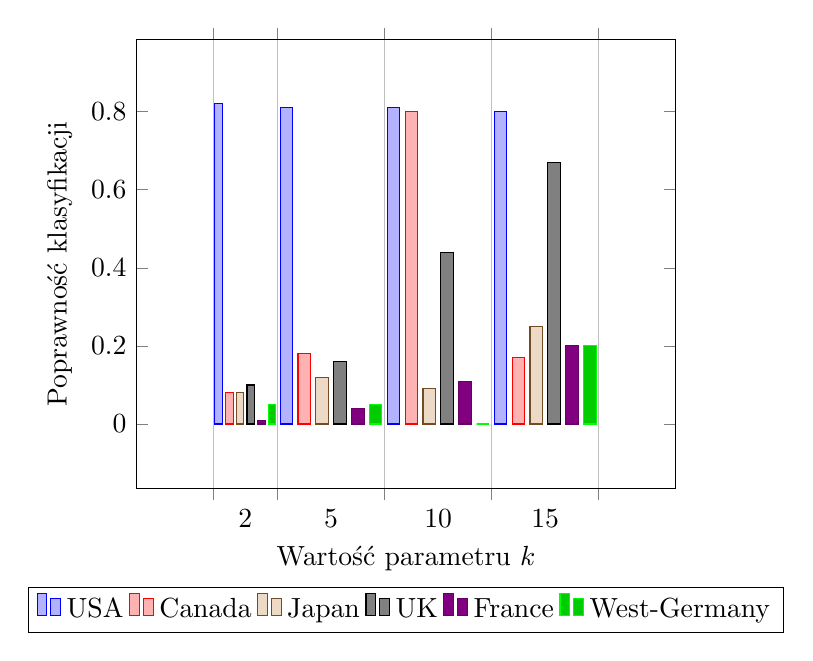
\begin{tikzpicture}
            \begin{axis}[
            x tick label style={
            /pgf/number format/1000 sep=},
            ylabel=Poprawność klasyfikacji,
            xlabel=Wartość parametru $k$,
            enlargelimits=0.2,
            legend style={at={(0.5,-0.22)},
            anchor=north,legend columns=-1},
            ybar interval=0.7,
            ]
                \addplot
                coordinates {
                (2,0.82)(5,0.81)(10,0.81)(15,0.80)(20,0.80)
                };

                \addplot
                coordinates {
                (2,0.08)(5,0.18)(10,0.8)(15,0.17)(20,0.5)
                };

                \addplot
                coordinates {
                (2,0.08)(5,0.12)(10,0.09)(15,0.25)(20,0.25)
                };

                \addplot
                coordinates {
                (2,0.10)(5,0.16)(10,0.44)(15,0.67)(20,0)
                };

                \addplot
                coordinates {
                (2,0.01)(5,0.04)(10,0.11)(15,0.20)(20,0)
                };

                \addplot
                coordinates {
                (2,0.05)(5,0.05)(10,0)(15,0.20)(20,0.20)
                };

                \legend{USA, Canada, Japan, UK, France, West-Germany}
            \end{axis}

        \end{tikzpicture}
    \end{center}
    \caption{Poprawność klasyfikacji etykiety dla wybranych wartości parametru
    $k$ dla kategorii $PLACES$ z użyciem metryki Czebyszewa.}
    \label{1_places_label_cz}
\end{figure}
\FloatBarrier
\subsection{Wyniki klasyfikacji dla kategorii $TOPICS$}
Klasyfikację przeprowadzono dla podanych w punkcie \ref{mat} danych. Zbiór danych jest znacznie mniejszy
od poprzedniego, zawiera on jedynie 173 elementy.

\begin{figure}[h!]
    \begin{center}
    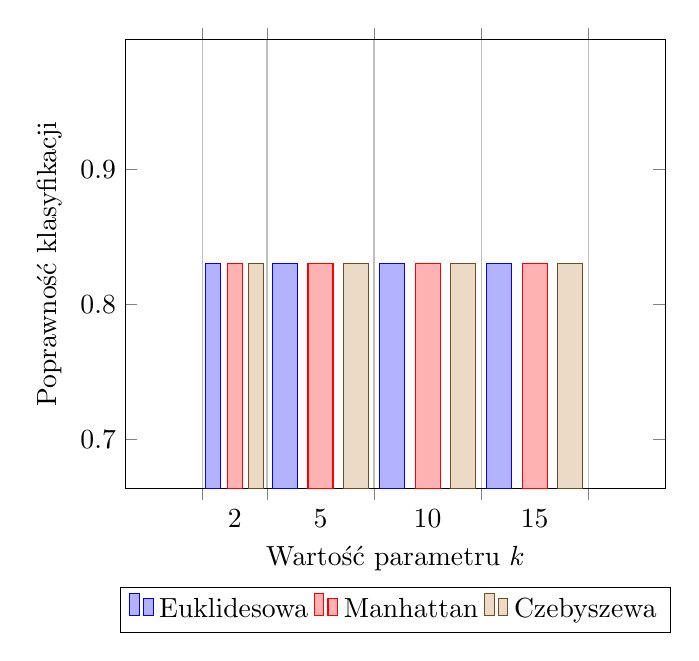
\begin{tikzpicture}
        \begin{axis}[
        x tick label style={
        /pgf/number format/1000 sep=},
        ylabel=Poprawność klasyfikacji,
        xlabel=Wartość parametru $k$,
        enlargelimits=0.2,
        legend style={at={(0.5,-0.22)},
        anchor=north,legend columns=-1},
        ybar interval=0.7,
        ]
            \addplot
            coordinates {
            (2,0.83)(5,0.83)(10,0.83)(15,0.83)(20,0.83)
            };

            \addplot
            coordinates {
            (2,0.83)(5,0.83)(10,0.83)(15,0.83)(20,0.83)
            };

            \addplot
            coordinates {
            (2,0.83)(5,0.83)(10,0.83)(15,0.83)(20,0.83)
            };

            \legend{Euklidesowa, Manhattan, Czebyszewa}
        \end{axis}

    \end{tikzpicture}
\end{center}
\caption{Poprawność klasyfikacji dla wybranych wartości parametru $k$ i zawartych metryk dla
kategorii $TOPICS$.}
\label{1_topics}
\end{figure}

\begin{figure}[h!]
    \begin{center}
        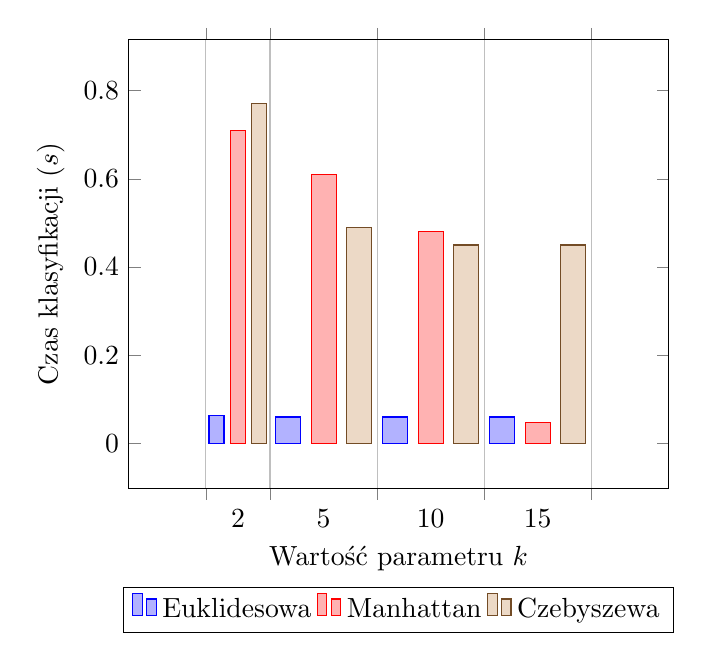
\begin{tikzpicture}
            \begin{axis}[
            x tick label style={
            /pgf/number format/1000 sep=},
            ylabel=Czas klasyfikacji ($s$),
            xlabel=Wartość parametru $k$,
            enlargelimits=0.2,
            legend style={at={(0.5,-0.22)},
            anchor=north,legend columns=-1},
            ybar interval=0.7,
            ]
                \addplot
                coordinates {
                (2,0.063)(5,0.06)(10,0.06)(15,0.06)(20,0.061)
                };

                \addplot
                coordinates {
                (2,0.71)(5,0.61)(10,0.48)(15,0.047)(20,0.044)
                };

                \addplot
                coordinates {
                (2,0.77)(5,0.49)(10,0.45)(15,0.45)(20,0.46)
                };

                \legend{Euklidesowa, Manhattan, Czebyszewa}
            \end{axis}

        \end{tikzpicture}
    \end{center}
    \caption{Czas klasyfikacji dla wybranych wartości parametru $k$ i zawartych metryk dla
    kategorii $TOPICS$.}
    \label{1_topics_time}
\end{figure}

\begin{figure}[h!]
    \begin{center}
        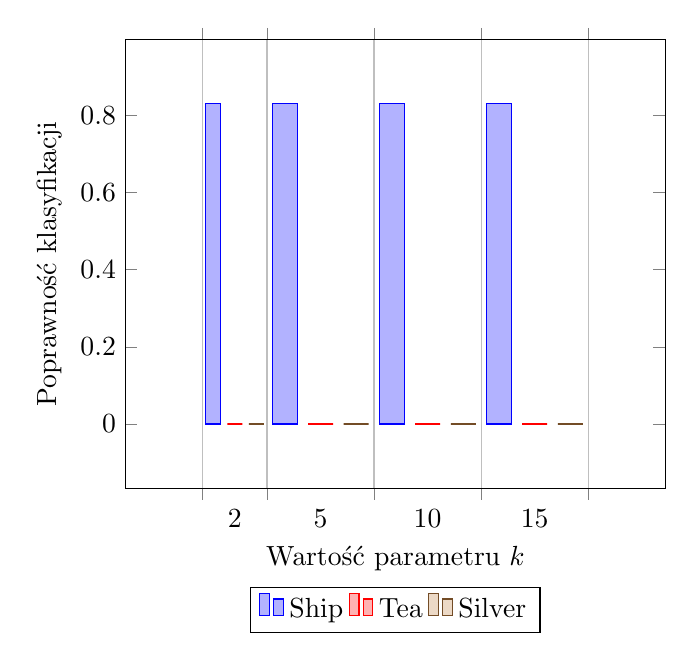
\begin{tikzpicture}
            \begin{axis}[
            x tick label style={
            /pgf/number format/1000 sep=},
            ylabel=Poprawność klasyfikacji,
            xlabel=Wartość parametru $k$,
            enlargelimits=0.2,
            legend style={at={(0.5,-0.22)},
            anchor=north,legend columns=-1},
            ybar interval=0.7,
            ]
                \addplot
                coordinates {
                (2,0.83)(5,0.83)(10,0.83)(15,0.83)(20,0.83)
                };

                \addplot
                coordinates {
                (2,0)(5,0)(10,0)(15,0)(20,0)
                };

                \addplot
                coordinates {
                (2,0)(5,0)(10,0)(15,0)(20,0)
                };

                \legend{Ship, Tea, Silver}
            \end{axis}

        \end{tikzpicture}
    \end{center}
    \caption{Poprawność klasyfikacji etykiety dla wybranych wartości parametru
    $k$ dla kategorii $TOPICS$ z użyciem metryki Euklidesowej.}
    \label{1_topics_label_euk}
\end{figure}

\begin{figure}[h!]
    \begin{center}
        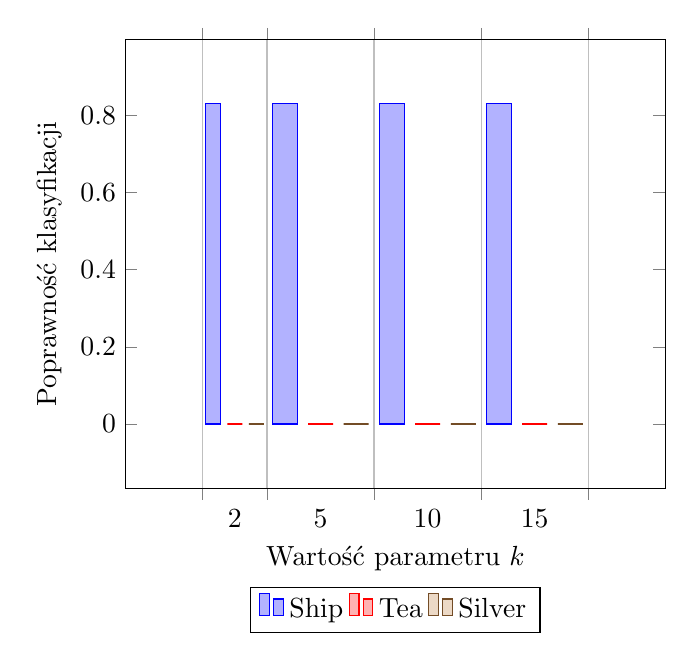
\begin{tikzpicture}
            \begin{axis}[
            x tick label style={
            /pgf/number format/1000 sep=},
            ylabel=Poprawność klasyfikacji,
            xlabel=Wartość parametru $k$,
            enlargelimits=0.2,
            legend style={at={(0.5,-0.22)},
            anchor=north,legend columns=-1},
            ybar interval=0.7,
            ]
                \addplot
                coordinates {
                (2,0.83)(5,0.83)(10,0.83)(15,0.83)(20,0.83)
                };

                \addplot
                coordinates {
                (2,0)(5,0)(10,0)(15,0)(20,0)
                };

                \addplot
                coordinates {
                (2,0)(5,0)(10,0)(15,0)(20,0)
                };

                \legend{Ship, Tea, Silver}
            \end{axis}

        \end{tikzpicture}
    \end{center}
    \caption{Poprawność klasyfikacji etykiety dla wybranych wartości parametru
    $k$ dla kategorii $TOPICS$ z użyciem metryki Manhattan.}
    \label{1_topics_label_man}
\end{figure}

\begin{figure}[h!]
    \begin{center}
        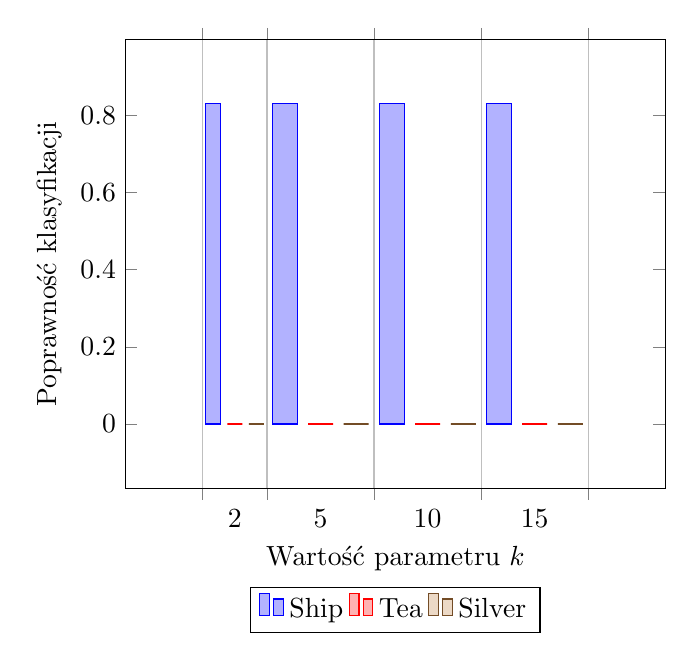
\begin{tikzpicture}
            \begin{axis}[
            x tick label style={
            /pgf/number format/1000 sep=},
            ylabel=Poprawność klasyfikacji,
            xlabel=Wartość parametru $k$,
            enlargelimits=0.2,
            legend style={at={(0.5,-0.22)},
            anchor=north,legend columns=-1},
            ybar interval=0.7,
            ]
                \addplot
                coordinates {
                (2,0.83)(5,0.83)(10,0.83)(15,0.83)(20,0.83)
                };

                \addplot
                coordinates {
                (2,0)(5,0)(10,0)(15,0)(20,0)
                };

                \addplot
                coordinates {
                (2,0)(5,0)(10,0)(15,0)(20,0)
                };

                \legend{Ship, Tea, Silver}
            \end{axis}

        \end{tikzpicture}
    \end{center}
    \caption{Poprawność klasyfikacji etykiety dla wybranych wartości parametru
    $k$ dla kategorii $TOPICS$ z użyciem metryki Czebyszewa.}
    \label{1_topics_label_cze}
\end{figure}

\FloatBarrier
\subsection{Wyniki klasyfikacji dla kategorii $TOPICS$ z użyciem ekstraktora TF}

\begin{figure}[h!]
    \begin{center}
        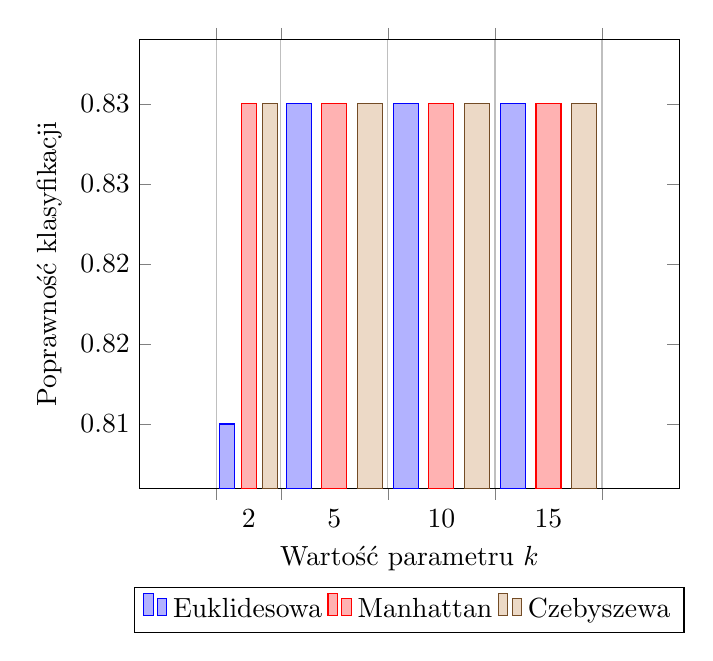
\begin{tikzpicture}
            \begin{axis}[
            x tick label style={
            /pgf/number format/1000 sep=},
            ylabel=Poprawność klasyfikacji,
            xlabel=Wartość parametru $k$,
            enlargelimits=0.2,
            legend style={at={(0.5,-0.22)},
            anchor=north,legend columns=-1},
            ybar interval=0.7,
            ]
                \addplot
                coordinates {
                (2,0.81)(5,0.83)(10,0.83)(15,0.83)(20,0.83)
                };

                \addplot
                coordinates {
                (2,0.83)(5,0.83)(10,0.83)(15,0.83)(20,0.83)
                };

                \addplot
                coordinates {
                (2,0.83)(5,0.83)(10,0.83)(15,0.83)(20,0.83)
                };

                \legend{Euklidesowa, Manhattan, Czebyszewa}
            \end{axis}

        \end{tikzpicture}
    \end{center}
    \caption{Poprawność klasyfikacji dla wybranych wartości parametru $k$ i zawartych metryk dla
    kategorii $TOPICS$ z użyciem ekstraktora TF.}
    \label{1_topics_tf}
\end{figure}

\begin{figure}[h!]
    \begin{center}
        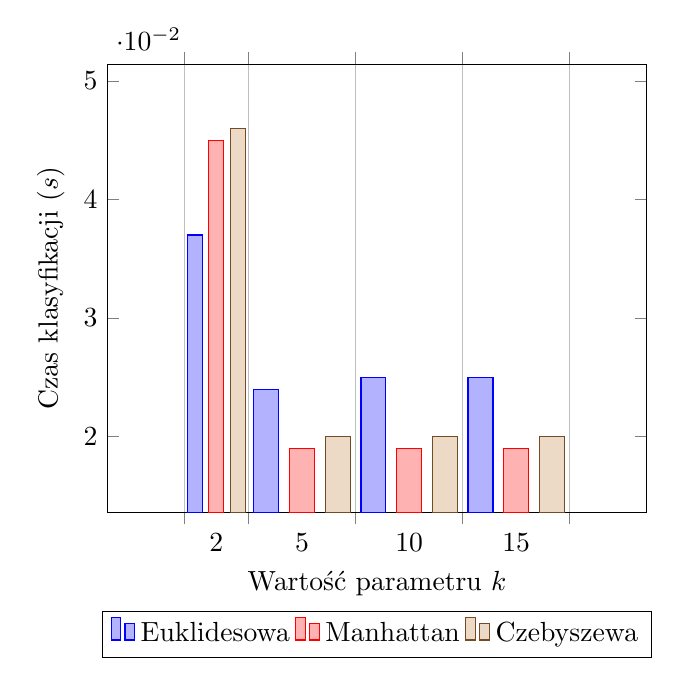
\begin{tikzpicture}
            \begin{axis}[
            x tick label style={
            /pgf/number format/1000 sep=},
            ylabel=Czas klasyfikacji ($s$),
            xlabel=Wartość parametru $k$,
            enlargelimits=0.2,
            legend style={at={(0.5,-0.22)},
            anchor=north,legend columns=-1},
            ybar interval=0.7,
            ]
                \addplot
                coordinates {
                (2,0.037)(5,0.024)(10,0.025)(15,0.025)(20,0.024)
                };

                \addplot
                coordinates {
                (2,0.045)(5,0.019)(10,0.019)(15,0.019)(20,0.019)
                };

                \addplot
                coordinates {
                (2,0.046)(5,0.02)(10,0.02)(15,0.02)(20,0.019)
                };

                \legend{Euklidesowa, Manhattan, Czebyszewa}
            \end{axis}

        \end{tikzpicture}
    \end{center}
    \caption{Czas wykonywania dla wybranych wartości parametru $k$ i zawartych metryk dla
    kategorii $TOPICS$ z użyciem ekstraktora TF.}
    \label{1_topics__tf_time}
\end{figure}


\FloatBarrier
\subsection{Wyniki klasyfikacji dla własnego zbioru}

\begin{figure}[h!]
    \begin{center}
        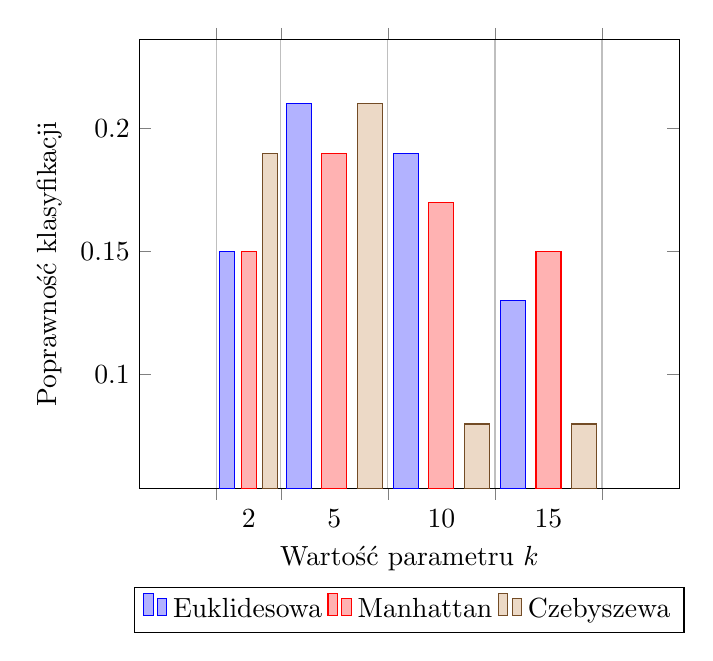
\begin{tikzpicture}
            \begin{axis}[
            x tick label style={
            /pgf/number format/1000 sep=},
            ylabel=Poprawność klasyfikacji,
            xlabel=Wartość parametru $k$,
            enlargelimits=0.2,
            legend style={at={(0.5,-0.22)},
            anchor=north,legend columns=-1},
            ybar interval=0.7,
            ]
                \addplot
                coordinates {
                (2,0.15)(5,0.21)(10,0.19)(15,0.13)(20,0.13)
                };

                \addplot
                coordinates {
                (2,0.15)(5,0.19)(10,0.17)(15,0.15)(20,0.1)
                };

                \addplot
                coordinates {
                (2,0.19)(5,0.21)(10,0.08)(15,0.08)(20,0.08)
                };

                \legend{Euklidesowa, Manhattan, Czebyszewa}
            \end{axis}

        \end{tikzpicture}
    \end{center}
    \caption{Poprawność klasyfikacji dla wybranych wartości parametru $k$ i zawartych metryk dla
    własnych tekstów.}
    \label{1_wlasny}
\end{figure}

\begin{figure}[h!]
    \begin{center}
        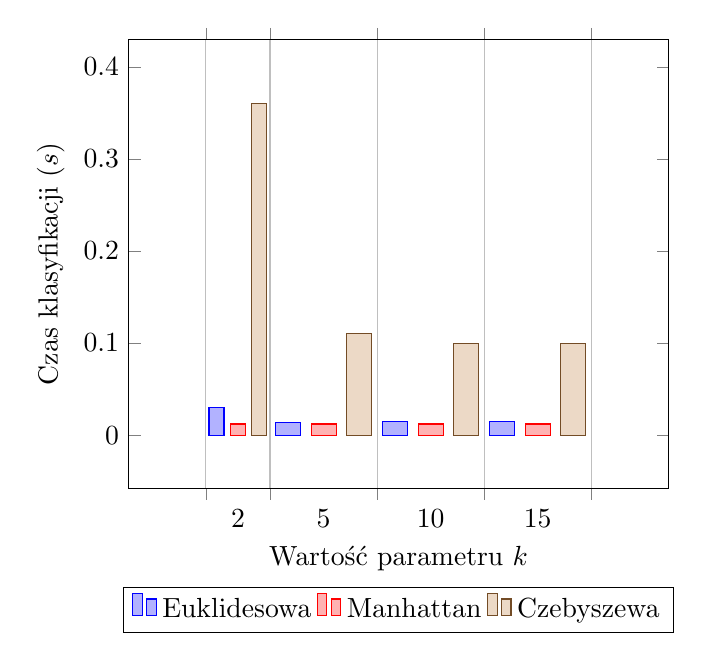
\begin{tikzpicture}
            \begin{axis}[
            x tick label style={
            /pgf/number format/1000 sep=},
            ylabel=Czas klasyfikacji ($s$),
            xlabel=Wartość parametru $k$,
            enlargelimits=0.2,
            legend style={at={(0.5,-0.22)},
            anchor=north,legend columns=-1},
            ybar interval=0.7,
            ]
                \addplot
                coordinates {
                (2,0.03)(5,0.014)(10,0.015)(15,0.015)(20,0.019)
                };

                \addplot
                coordinates {
                (2,0.012)(5,0.012)(10,0.012)(15,0.012)(20,0.012)
                };

                \addplot
                coordinates {
                (2,0.36)(5,0.11)(10,0.1)(15,0.1)(20,0.1)
                };

                \legend{Euklidesowa, Manhattan, Czebyszewa}
            \end{axis}

        \end{tikzpicture}
    \end{center}
    \caption{Czas wykonywania dla wybranych wartości parametru $k$ i zawartych metryk dla
    własnych tekstów.}
    \label{1_wlasny_time}
\end{figure}

\begin{figure}[h!]
    \begin{center}
        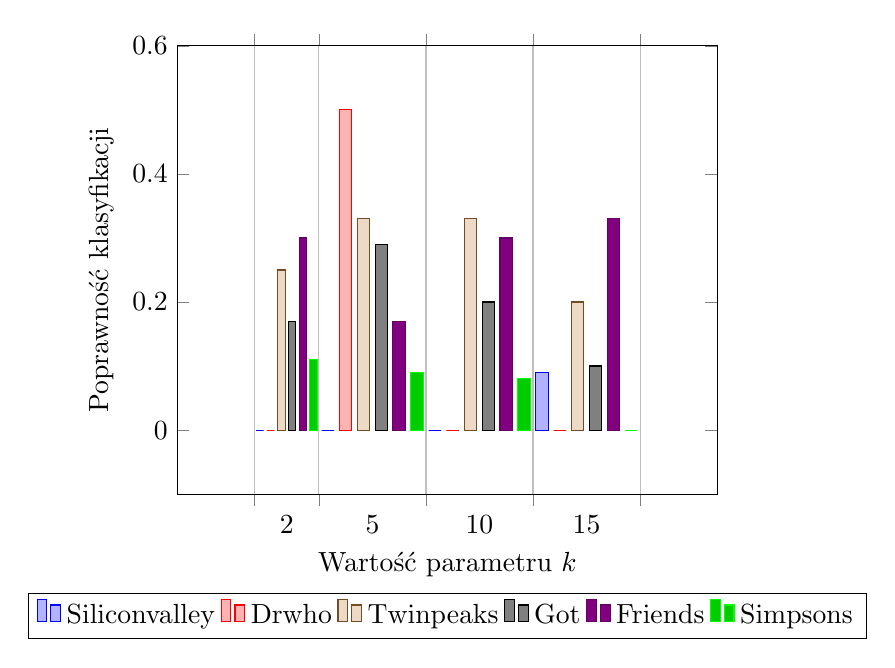
\begin{tikzpicture}
            \begin{axis}[
            x tick label style={
            /pgf/number format/1000 sep=},
            ylabel=Poprawność klasyfikacji,
            xlabel=Wartość parametru $k$,
            enlargelimits=0.2,
            legend style={at={(0.5,-0.22)},
            anchor=north,legend columns=-1},
            ybar interval=0.7,
            ]
                \addplot
                coordinates {
                (2,0)(5,0)(10,0)(15,0.09)(20,0.11)
                };

                \addplot
                coordinates {
                (2,0)(5,0.50)(10,0)(15,0)(20,0)
                };

                \addplot
                coordinates {
                (2,0.25)(5,0.33)(10,0.33)(15,0.20)(20,0.18)
                };

                \addplot
                coordinates {
                (2,0.17)(5,0.29)(10,0.20)(15,0.1)(20,0.09)
                };

                \addplot
                coordinates {
                (2,0.30)(5,0.17)(10,0.30)(15,0.33)(20,0.33)
                };

                \addplot
                coordinates {
                (2,0.11)(5,0.09)(10,0.08)(15,0)(20,0)
                };

                \legend{Siliconvalley, Drwho, Twinpeaks, Got, Friends, Simpsons}
            \end{axis}

        \end{tikzpicture}
    \end{center}
    \caption{Poprawność klasyfikacji etykiety dla wybranych wartości parametru
    $k$ dla własnych tekstów z użyciem metryki Euklidesowej.}
    \label{1_wlasny_label_euk}
\end{figure}

\begin{figure}[h!]
    \begin{center}
        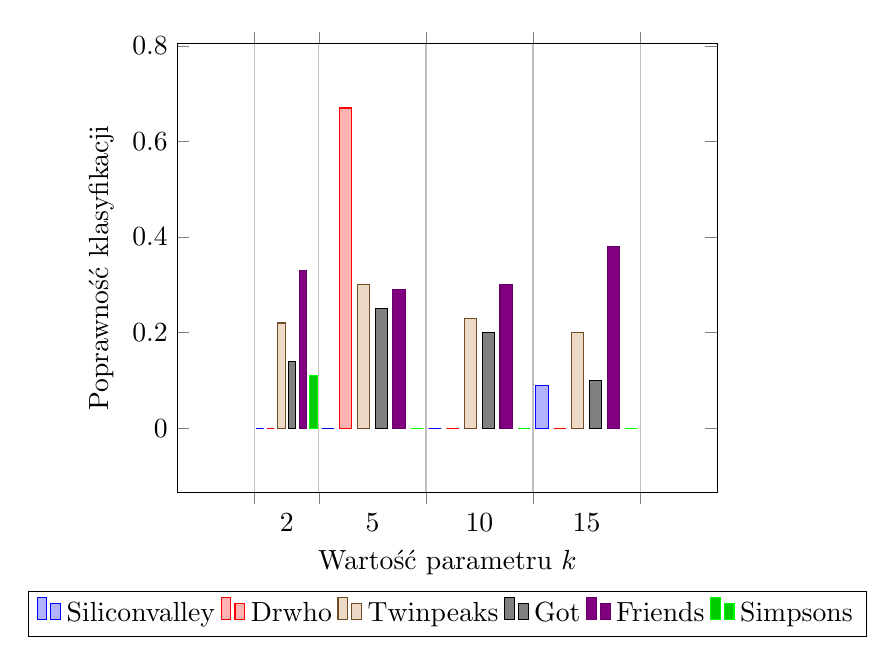
\begin{tikzpicture}
            \begin{axis}[
            x tick label style={
            /pgf/number format/1000 sep=},
            ylabel=Poprawność klasyfikacji,
            xlabel=Wartość parametru $k$,
            enlargelimits=0.2,
            legend style={at={(0.5,-0.22)},
            anchor=north,legend columns=-1},
            ybar interval=0.7,
            ]
                \addplot
                coordinates {
                (2,0)(5,0)(10,0)(15,0.09)(20,0.11)
                };

                \addplot
                coordinates {
                (2,0)(5,0.67)(10,0)(15,0)(20,0)
                };

                \addplot
                coordinates {
                (2,0.22)(5,0.30)(10,0.23)(15,0.20)(20,0.17)
                };

                \addplot
                coordinates {
                (2,0.14)(5,0.25)(10,0.2)(15,0.1)(20,0.08)
                };

                \addplot
                coordinates {
                (2,0.33)(5,0.29)(10,0.30)(15,0.38)(20,0.25)
                };

                \addplot
                coordinates {
                (2,0.11)(5,0)(10,0)(15,0)(20,0)
                };

                \legend{Siliconvalley, Drwho, Twinpeaks, Got, Friends, Simpsons}
            \end{axis}

        \end{tikzpicture}
    \end{center}
    \caption{Poprawność klasyfikacji etykiety dla wybranych wartości parametru
    $k$ dla własnych tekstów z użyciem metryki Manhattan.}
    \label{1_wlasne_label_man}
\end{figure}

\begin{figure}[h!]
    \begin{center}
        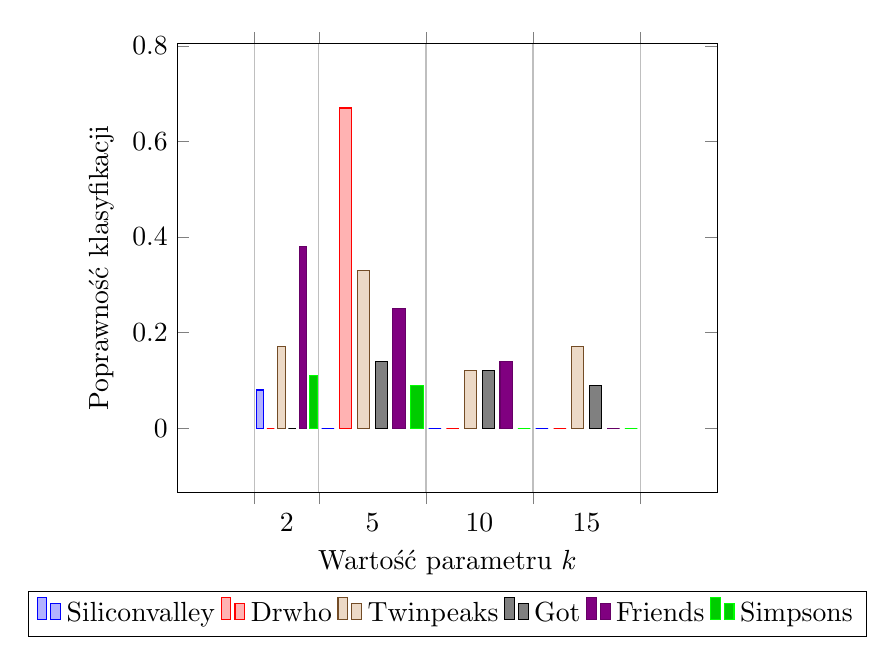
\begin{tikzpicture}
            \begin{axis}[
            x tick label style={
            /pgf/number format/1000 sep=},
            ylabel=Poprawność klasyfikacji,
            xlabel=Wartość parametru $k$,
            enlargelimits=0.2,
            legend style={at={(0.5,-0.22)},
            anchor=north,legend columns=-1},
            ybar interval=0.7,
            ]
                \addplot
                coordinates {
                (2,0.08)(5,0)(10,0)(15,0)(20,0)
                };

                \addplot
                coordinates {
                (2,0)(5,0.67)(10,0)(15,0)(20,0)
                };

                \addplot
                coordinates {
                (2,0.17)(5,0.33)(10,0.12)(15,0.17)(20,0.17)
                };

                \addplot
                coordinates {
                (2,0)(5,0.14)(10,0.12)(15,0.09)(20,0.18)
                };

                \addplot
                coordinates {
                (2,0.38)(5,0.25)(10,0.14)(15,0)(20,0)
                };

                \addplot
                coordinates {
                (2,0.11)(5,0.09)(10,0)(15,0)(20,0)
                };

                \legend{Siliconvalley, Drwho, Twinpeaks, Got, Friends, Simpsons}
            \end{axis}

        \end{tikzpicture}
    \end{center}
    \caption{Poprawność klasyfikacji etykiety dla wybranych wartości parametru
    $k$ dla własnych tekstów z użyciem metryki Czebyszewa.}
    \label{1_wlasny_label_cze}
\end{figure}


\FloatBarrier
\subsection{Wpływ rozmiaru zbioru uczącego na skuteczność klasyfikacji}


\begin{figure}[h!]
    \begin{center}
        \begin{tikzpicture}
%            \begin{axis}[
%            x tick label style={
%            /pgf/number format/10000 sep=},
%            ylabel=Poprawność klasyfikacji,
%            xlabel=Rozmiar zbioru uczącego (\%),
%            xticklabels={,,,,,},
%            enlargelimits=0.2,
%            legend style={at={(0.5,-0.25)},
%            anchor=north,legend columns=-1},
%            ybar interval=0.7,
%            ]
%                \addplot
%                coordinates {
%                (1,0.65)(0,0)(0,0)(0,0)(0,0)(0,0)
%                };
%
%                \addplot
%                coordinates {
%                (1,0.46)(0,0)(0,0)(0,0)(0,0)(0,0)
%                };
%
%                \addplot
%                coordinates {
%                (1,0.42)(0,0)(0,0)(0,0)(0,0)(0,0)
%                };
%
%                \addplot
%                coordinates {
%                (1,0.52)(0,0)(0,0)(0,0)(0,0)(0,0)
%                };
%
%                \addplot
%                coordinates {
%                (1,0.52)(0,0)(0,0)(0,0)(0,0)(0,0)
%                };
%
%                \addplot
%                coordinates {
%                (1,0.48)(0,0)(0,0)(0,0)(0,0)(0,0)
%                };
%
%                \addplot
%                coordinates {
%                (1,0.4)(0,0)(0,0)(0,0)(0,0)(0,0)
%                };
%
%                \addplot
%                coordinates {
%                (1,0.38)(0,0)(0,0)(0,0)(0,0)(0,0)
%                };
%
%                \addplot
%                coordinates {
%                (1,0.27)(0,0)(0,0)(0,0)(0,0)(0,0)
%                };
%
%                \legend{90, 80, 70, 60, 50, 40, 30, 20, 10}
%            \end{axis}

            \begin{axis}[
            ylabel=Poprawność klasyfikacji ($\%$),
            xlabel=Rozmiar zbioru uczącego (\%),
            symbolic x coords={90, 80, 70, 60, 50, 40, 30, 20, 10},
            xtick=data]
                \addplot[ybar,fill=black!30!green] coordinates {
                (90,0.65)
                (80,0.46)
                (70,0.42)
                (60,0.52)
                (50,0.52)
                (40,0.48)
                (30,0.4)
                (20,0.38)
                (10,0.27)
                };
            \end{axis}

        \end{tikzpicture}
    \end{center}
    \caption{Poprawność klasyfikacji dla danego podziału zbioru.}
    \label{podzial_zbioru}
\end{figure}

\FloatBarrier
\subsection{Wpływ miary podobieństwa słów na poprawnośc klasyfikacji}

\begin{figure}[h!]
    \begin{center}
        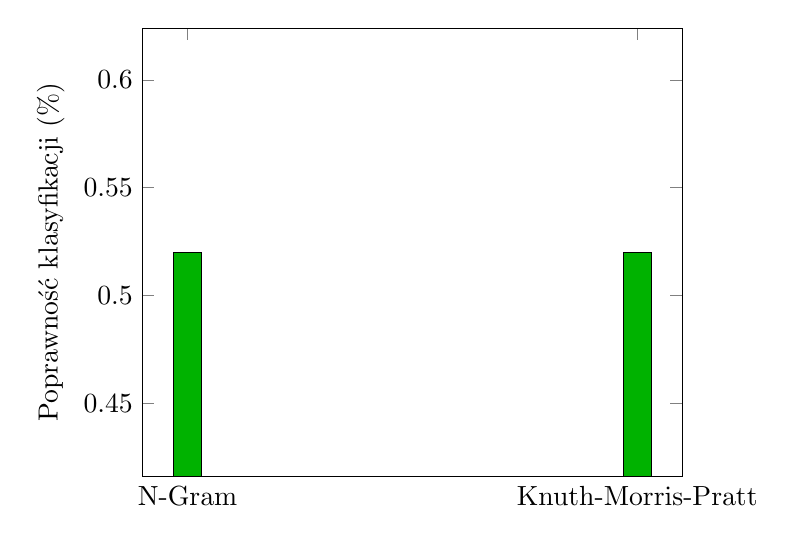
\begin{tikzpicture}
%            \begin{axis}[
%            x tick label style={
%            /pgf/number format/10000 sep=},
%            ylabel=Poprawność klasyfikacji,
%            xlabel=Miara podobieństwa słów,
%            xticklabels={,},
%            enlargelimits=0.2,
%            legend style={at={(0.5,-0.25)},
%            anchor=north,legend columns=-1},
%            ybar interval=0.7,
%            ]
%                \addplot
%                coordinates {
%                (1,0.52)(0,0)
%                };
%
%                \addplot
%                coordinates {
%                (1,0.52)(0,0)
%                };
%
%                \legend{N-Gram, Knuth-Morris-Pratt}
%            \end{axis}

            \begin{axis}[
            ylabel=Poprawność klasyfikacji ($\%$),
            symbolic x coords={N-Gram, Knuth-Morris-Pratt},
            xtick=data]
                \addplot[ybar,fill=black!30!green] coordinates {
                (N-Gram,0.52)
                (Knuth-Morris-Pratt,0.52)
                };
            \end{axis}

        \end{tikzpicture}
    \end{center}
    \caption{Poprawność klasyfikacji dla miar podobieństwa słów.}
    \label{popr_miara_prawdo}
\end{figure}

\begin{figure}[h!]
    \begin{center}
        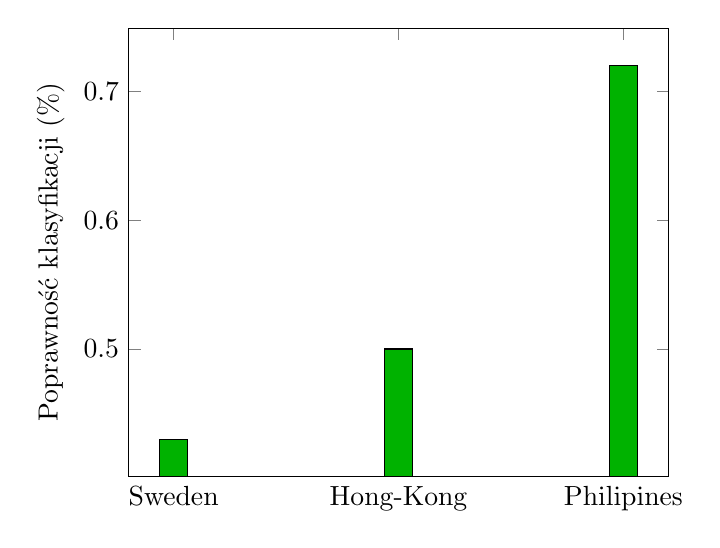
\begin{tikzpicture}
%            \begin{axis}[
%            x tick label style={
%            /pgf/number format/1000 sep=},
%            ylabel=Poprawność klasyfikacji,
%            xlabel=Etykieta,
%            xticklabels={,,},
%            enlargelimits=0.2,
%            legend style={at={(0.5,-0.22)},
%            anchor=north,legend columns=-1},
%            ybar interval=0.7,
%            ]
%                \addplot
%                coordinates {
%                (1,0.43)(0,0)(0,0)
%                };
%
%                \addplot
%                coordinates {
%                (1,0.50)(0,0)(0,0)
%                };
%
%                \addplot
%                coordinates {
%                (1,0.72)(0,0)(0,0)
%                };
%
%                \legend{Sweden, Hong-Kong, Philipines}
%            \end{axis}

            \begin{axis}[
            ylabel=Poprawność klasyfikacji ($\%$),
            symbolic x coords={Sweden, Hong-Kong, Philipines},
            xtick=data]
                \addplot[ybar,fill=black!30!green] coordinates {
                (Sweden,0.43)
                (Hong-Kong,0.50)
                (Philipines,0.72)

                };
            \end{axis}

        \end{tikzpicture}
    \end{center}
    \caption{Poprawność klasyfikacji etykiet dla miary N-Gramów.}
    \label{ngram_popraw_ngram}
\end{figure}

\begin{figure}[h!]
    \begin{center}
        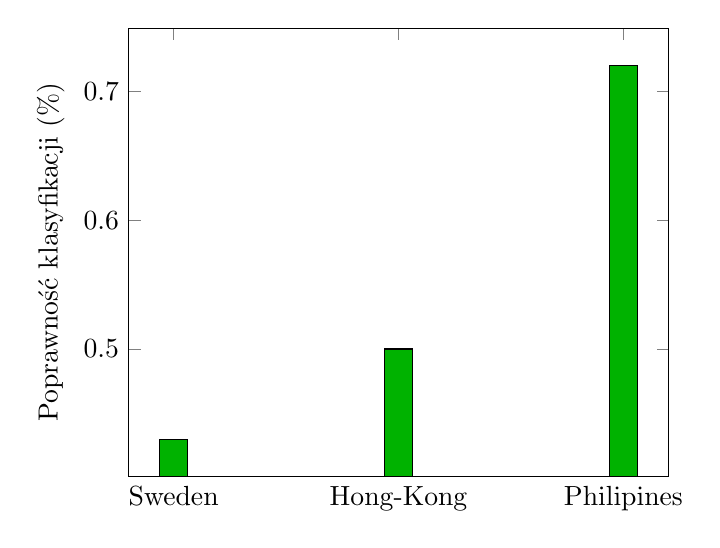
\begin{tikzpicture}
%            \begin{axis}[
%            x tick label style={
%            /pgf/number format/10000 sep=},
%            ylabel=Poprawność klasyfikacji,
%            xlabel=Etykieta,
%            xticklabels={,,},
%            enlargelimits=0.2,
%            legend style={at={(0.5,-0.25)},
%            anchor=north,legend columns=-1},
%            ybar interval=0.7,
%            ]
%                \addplot
%                coordinates {
%                (1,0.43)(0,0)(0,0)
%                };
%
%                \addplot
%                coordinates {
%                (1,0.50)(0,0)(0,0)
%                };
%
%                \addplot
%                coordinates {
%                (1,0.72)(0,0)(0,0)
%                };
%
%                \legend{Sweden, Hong-Kong, Philipines}
%            \end{axis}

            \begin{axis}[
            ylabel=Poprawność klasyfikacji ($\%$),
            symbolic x coords={Sweden, Hong-Kong, Philipines},
            xtick=data]
                \addplot[ybar,fill=black!30!green] coordinates {
                (Sweden,0.43)
                (Hong-Kong,0.50)
                (Philipines,0.72)

                };
            \end{axis}

        \end{tikzpicture}
    \end{center}
    \caption{Poprawność klasyfikacji etykiet dla miary Knutta-Morrisa-Pratta.}
    \label{ngram_popraw_knutt}
\end{figure}

\FloatBarrier
\subsection{Wpływ danej cechy na poprawność klasyfikacji oraz jej czas trwania}
Dla lepszej czytelności wykresów wprowadziliśmy oznaczenia odpowiadające danym cechom przedstawionym
poniżej.
\begin{itemize}
    \item $A$ - Gęstość występowania słów kluczowych
    \item $B$ - Występowanie słowa kluczowego
    \item $C$ - Liczba wystąpień słów kluczowych
    \item $D$ - Odległość słowa kluczowego od początku tekstu
    \item $E$ - Liczba wszystkich słów w dokumencie
    \item $F$ - Pierwsze słowo kluczowe z dokumentu
    \item $G$ - Suma wyspień słów kluczowych w dokumencie
    \item $H$ - Średnia odległość słów kluczowych w dokumencie
    \item $I$ - Najczęściej występujęce słowo kluczowe
    \item $AL$ - Wszystkie cechy
\end{itemize}

\begin{figure}[h!]
    \begin{center}
        \begin{tikzpicture}
            \begin{axis}[
            ylabel=Poprawność klasyfikacji ($\%$),
            xlabel=Pominięta cecha,
            symbolic x coords={A,B,C,D,E,F,G,H,I,AL},
            xtick=data]
                \addplot[ybar,fill=black!30!green] coordinates {
                (A,0.47)
                (B,0.47)
                (C,0.47)
                (D,0.48)
                (E,0.48)
                (F,0.47)
                (G,0.47)
                (H,0.47)
                (I,0.47)
                (AL,0.47)
                };
            \end{axis}

        \end{tikzpicture}
    \end{center}
    \caption{Poprawność klasyfikacji z pominięciem danej cechy.}
    \label{cecha_poprawnosc}
\end{figure}

\begin{figure}
    \begin{center}
        \begin{tikzpicture}
            \begin{axis}[
            ylabel=Czas klasyfikacji ($s$),
            xlabel=Pominięta cecha,
            symbolic x coords={A,B,C,D,E,F,G,H,I,AL},
            xtick=data]
                \addplot[ybar,fill=black!30!green] coordinates {
                (A,15.154)
                (B,14.172)
                (C,14.706)
                (D,9.905)
                (E,14.259)
                (F,14.093)
                (G,14.11)
                (H,10.203)
                (I,14.232)
                (AL,14.492)
                };
            \end{axis}
        \end{tikzpicture}
    \end{center}
    \caption{Czas klasyfikacji z pominięciem danej cechy.}
    \label{cecha_czas}
\end{figure}

\FloatBarrier
\subsection{Wpływ parametru $N$ w metodzie N-Gramów na poprawność klasyfikacji}
\begin{figure}[h!]
    \begin{center}
        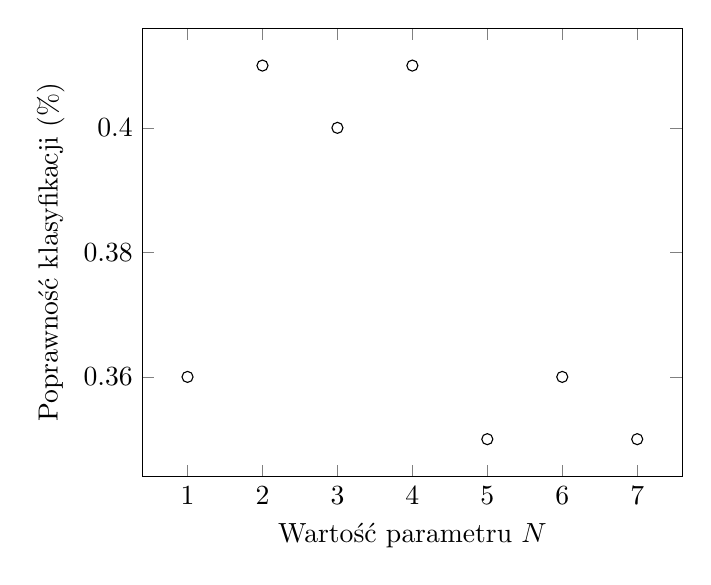
\begin{tikzpicture}
            \begin{axis}[
            ylabel=Poprawność klasyfikacji ($\%$),
            xlabel=Wartość parametru $N$,%
            scatter/classes={%
            a={mark=o,draw=black}}]
                \addplot[scatter,only marks,%
                scatter src=explicit symbolic]%
                table[meta=label] {
                x y label
                1 0.36 a
                2 0.41 a
                3 0.4 a
                4 0.41 a
                5 0.35 a
                6 0.36 a
                7 0.35 a

                };
            \end{axis}

        \end{tikzpicture}
    \end{center}
    \caption{Poprawność klasyfikacji w zależności od parametru $N$ w metodzie N-Gramów.}
    \label{n_gramn}
\end{figure}

\begin{figure}[h!]
    \begin{center}
        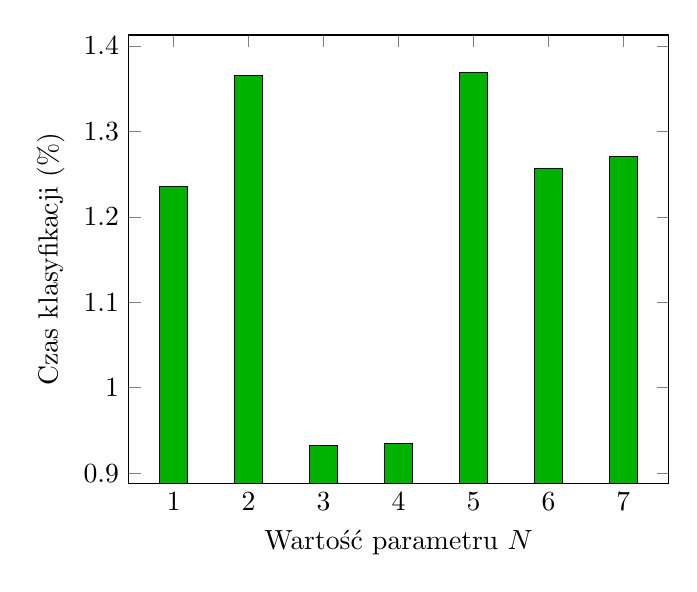
\begin{tikzpicture}
            \begin{axis}[
            ylabel=Czas klasyfikacji ($\%$),
            xlabel=Wartość parametru $N$,
            symbolic x coords={1,2,3,4,5,6,7},
            xtick=data]
                \addplot[ybar,fill=black!30!green] coordinates {
                (1,1.235)
                (2,1.365)
                (3,0.932)
                (4,0.935)
                (5,1.369)
                (6,1.256)
                (7,1.271)
                };
            \end{axis}

        \end{tikzpicture}
    \end{center}
    \caption{Czas klasyfikacji w zależności od parametru $N$ w metodzie N-Gramów.}
    \label{n_gramn_czas}
\end{figure}


%{\color{blue}
%W tej sekcji należy zaprezentować, dla każdego przeprowadzonego eksperymentu,
%kompletny zestaw wyników w postaci tabel, wykresów itp. Powinny być one tak
%ponazywane, aby było wiadomo, do czego się odnoszą. Wszystkie tabele i wykresy
%należy oczywiście opisać (opisać co jest na osiach, w kolumnach itd.) stosując
%się do przyjętych wcześniej oznaczeń. Nie należy tu komentować i interpretować
%wyników, gdyż miejsce na to jest w kolejnej sekcji. Tu również dobrze jest
%wprowadzić oznaczenia (tabel, wykresów) aby móc się do nich odwoływać
%poniżej.}

\section{Dyskusja}
Na podstawie przeprowadzonych badań klasyfikacji tekstów można stwierdzić, że klasyfikacja teskstów
jest złożonym zagadnieniem. W związku z tym dzielimy obszary badań na kilka kategorii.

\subsection{Wpływ parametru $k$}
Przeprowadzone badania pozwalają stwierdzić, że wartośc parametru $k$ ma znaczy wpływ na poprawność
klasyfikacji, lecz do pewnego momentu. Na podstawie rysunku \ref{1_places} można stwierdzić, że
zbyt niska wartość parametru $k$ negatywnie wpływa na poprawnośc klasyfikacji. Podczas klasyfikacji
dla kategorii $PLACES$ i $k=2$ skuteczność dla każdej metryki wyniosła $64\%$. Natomiast, jak wynika
z rysunku \ref{1_topics}, dla
kategorii $TOPICS$ poprawność klasyfikacji wyniosła $83\%$ i nie była użależniona od wartości $k$.
Wyniki przedstawione na rusynku \ref{1_wlasny} wskazują na niski próg poprawności dla własnych tekstów.
Dla parametru $k=5$ wyniki były najlepsze.


\subsection{Wpływ metryki}
Pomiędzy metrykami wykorzystanymi w klasyfikacji kategorii $PLACES$ oraz $TOPICS$ nie wykazano
różnic ze względu na
poprawność klasyfikacji co przedstawia rysunek \ref{1_places} oraz \ref{1_topics}. Badając własny
zbiór tekstów (rysunek \ref{1_wlasny}) zaobserwowano, że wpływ metryki jest znacznie większy niż w poprzednich przypadkach.
Metryka czebyszewa klasyfikuje obiekty w sposób mniej dokładny niż pozostałe.
Znaczące róznice
pojawiają się z czasie klasyfikacji. Metryka Euklidesowa zarówno dla kategorii $PLACES$ jak i $TOPICS$
wykazuje złożoność obliczeniową liniową co można zaobserwować na rysunkach: \ref{1_places_time},
\ref{1_topics_time}. Należy pamiętać że wyniki te są najmniej miarodajne ponieważ mogą się znacząco
różnić w zależności od zasobów sprzętowych, które są dostępne w danym momencie.

\subsection{Liczebność zbiorów}
Badania wykazały, że na poprawność klasyfikacji znaczący wpływ ma liczebność zbiorów. W przypadku
kiedy dana etykieta znacząco przeważa liczebnością pozostałe, wyniki klasyfikacji dla pozostałych
etykiet będą niskie. Spowodowane jest to znikomą liczbą pozostałych etykiet w zbiorze uczącym.
Liczebność zbiorów pokazują rysunki \ref{licz_places}, \ref{licz_topics} oraz \ref{licz_wlasny}.

\subsection{Wpływ podziału zbiorów}
Z rysunku \ref{podzial_zbioru} można odczytać, że dla podziału zbioru w
stosunku $30\%$ (zbiór uczący) do $70\%$ (zbiór testowy) oraz niższych wartości dla zbioru uczącego
skuteczność klasyfikacji uległa pogorszeniu. Podobnych obserwacji można dokonać w przypadku, gdy
zbiór uczący stanowi $70\%$
klasyfikowanych obiektów.

\subsection{Wpływ miary podobieństwa}
Rysunek \ref{popr_miara_prawdo} przedstawia takie same wartości poprawności klasyfikacji dla obydwu
miar podobieństwa słów. Nie wykazano różnic na poziomie poprawności klasyfikacji dla poszczególnych
etykiet (rysunki \ref{ngram_popraw_ngram}, \ref{ngram_popraw_knutt}). Zróżnicowanie czasu klasyfikacji
w przypadku obydwu miar podobieństwa było na tyle małe, że nie byliśmy w stanie określić która
miara jest optymalna. Wynika to z odmiennego czasu wykonywania klasyfikacji przy każdym uruchomieniu.

\subsection{Wpływ danych cech}
Badanie ma na celu sprawdzenie uniwersalnych metod ekstrakcji cech i ich wpływ na skuteczność
klasyfikacji (rysunki \ref{cecha_poprawnosc}, \ref{cecha_czas}). Przeprowadzone badania wskazują,
że pominięcie cechy w postaci liczby wysąpień słowa kluczowego lub odległości słowa kluczowego od początku tekstu
nieznacznie wpływa na zwiększenie poprawności klasyfikacji. Ponadto wyłączając cechę odległości słowa
kluczowego od początku tekstu oprócz lepszej klasyfikacji zyskujemy zmniejszony jej czas trwania.
Biorąc pod uwagę cechę średniej odległości słów kluczowych od początku tekstu zyskujemy zmniejszony
czas klasyfikacji jednocześnie nie zwiększając jej poprawności. W przypadku pozostałych cech nie można
jednoznacznie swierdzić przewagi jednej cechy nad drugą, ponieważ podobnie jak w trakcie badania wpływu
metryki występuje tu różnica w czasie wykonania zależna od zasobów sprzętowych dostępnych w danym momencie.

\subsection{Wpływ parametru $N$}
Z rysunku \ref{n_gramn} wynika, że dla parametrów $N$ z zakresu $<2;4>$ wyniki klasyfikacji były najlepsze.
Wartość parametru powyżej lub poniżej podanego zakresu negatywnie wpływała na poprawność klasyfikacji.
Nie zaobserwowano znaczących różnic w czasie działania klasyfikacji. Różnice w czasie klasyfikacji
na poziomie 400ms nie są wystarczające aby swierdzić przewagę danej konfiguracji.

\subsection{Wpływ ekstraktora TF}
Podczas badania dotyczącego zmiany ekstraktora słów kluczowych (rysunek \ref{1_topics_tf}) z
algorytmu TF-IDF na algorytm TF,
nie wykazano znaczących różnic w poprawności klasyfikacji w stosunku do uprzednio
wykorzystywanego ekstraktora. Natomiast jak wynika z rysunku \ref{1_topics__tf_time} czas klasyfikacji
uległ nieznacznej poprawie.
%Klasyfikacja tekstów jest znacznie bardziej złożona niż mogło się to w pierwszej chwili wydawać.
%Aby dokonać poprawnej klasyfikacji należy uprzednio przeanalizować badane teksty pod kątem języka
%w, którym zostały napisane. W zależności od typu tekstu należy dobrać odpowiednie ekstraktory cech.
%Zadajemy sobie sprawę, iż badane przez nas dokumenty mają charakter artykułów z gazet. Dla danego typu
%badanego tekstu cecha odległości słów kluczowych od początku tekstu będzie kluczowa w poprawnej
%klasyfikacji. Natomiast na przykład dla opowiadania istotność tej cechy na tle innych znacząco zmaleje.
%Użyty w badaniu wektor cech składający się zarówno z wartości metajęzykowych (czyli takich dla, których
%znaczenie mają jedynie położenie danego słowa w tekście czy liczba liter składowych) oraz wartości
%semantycznych (takich, które zwracają szczególną uwagę na budowę słowa), pozwala na dokładniejsze
%zbadanie tekstu bez względu na to jak został on zbudowany. Stwierdzenie to można smiało postawić
%zwracając uwagę na wykres \ref{1_places} na, którym tylko dla metryki $Manhattan$ przy wartości
%parametu $k=10$ poprawność klasyfikacji była nieznacznie wyższa. W pozostałych przypadkach poprawność
%klasyfikacji nie zależała od zastosowanej metryki liczenia odległości.
%
%\\Podsumowywując wyniki czasu działania algorytmu na wykresie \ref{1_places_time} można zaobserwować
%nieznacznie różniący się czas wykonywania dla metryki Euklideswej bez względu na wartość parametru $k$.
%W przypadku metryki Czebyszewa czas wykonywania zwiększał się wraz ze wzrostem parametru.
%Z uwagi na podobny czas działania dla wszystkich przebadanych parametrów metryka Euklidesowa
%jest najbardziej uniwersalna.
%
%\\Odnośnie wykresów pokazujących poprawność klasyfikacji (wykresy \ref{1_places_label_eucli}
%\ref{1_places_label_man} \ref{1_places_label_cz}) dla poszczególnych etykiet zaobserwować można
%niepokojącą tendencję do poprawności klasyfikacji jedynie etykiety dla, której liczba artykułów
%znacząco przewyższała liczbę pozostałych. Bez względu na parametr $k$ dla etykiety $USA$ znacząca
%większość artykułów została sklasyfikowana poprawnie. Przyczyną tego jest przeważająca większość
%artykułów o tej kategorii. Aby uzyskać większą poprawność klasyfikacji
%dla pozostałych etykiet należało by znormalizować zbiór testowy tak aby znajdowały się z nim
%zbliżone ilości artykułów o tych etykietach które chcemy klasyfikować.
%
%\\Parametr $k$ nieznacznie wpływa na poprawność klasyfikacji dla etykiet ze znaczą ilością wystąpień.
%Jednakże im parametr $k$ jest większy tym poprawność klasyfikacji nieznacznie spada.
%
%\\Przyglądając się wynikom klasyfikacji dla tagu $TOPICS$ można ponownie stwierdzić, że metoda
%Euklidesowa do liczenia odległości jest najszybsza (wykres \ref{1_topics_time}). Pomimo tego, że
%każde badanie wykonywało się krócej niż sekundę. Szybkość metody Euklidesowej nie wpływa w żaden
%sposób na poprawność klasyfikacji co pokazują wykresy: \ref{1_topics_label_euk},
%\ref{1_topics_label_man}, \ref{1_topics_label_cze}. Ponownie jak w poprzednim badaniu poprawność
%klasyfikacji dla etykiet z nieznaczącą liczbą wystąpień w zbiorze uczącym jest znikoma.

%{\color{blue}
%Sekcja ta powinna zawierać dokładną interpretację uzyskanych wyników
%eksperymentów wraz ze szczegółowymi wnioskami z nich płynącymi. Najcenniejsze
%są, rzecz jasna, wnioski o charakterze uniwersalnym, które mogą być istotne
%przy innych, podobnych zadaniach. Należy również omówić i wyjaśnić wszystkie
%napotakane problemy (jeśli takie były). Każdy wniosek powinien mieć poparcie
%we wcześniej przeprowadzonych eksperymentach (odwołania do konkretnych
%wyników). Jest to jedna z najważniejszych sekcji tego sprawozdania, gdyż
%prezentuje poziom zrozumienia badanego problemu.}
\section{Wnioski}



%Stworzenie systemu klasyfikującego teksty jest zagodnieniem znacznie szerszym niż mogło się to z początku
%wydawać. Wymaga zgłębienia tajników budowy tekstów jak i samych wyrazów. Ilość kombinacji w przypadku klasyfikacji
%tekstów jest tak ogromna, że można posiwięcić temu zagadnieniu całe życie. W naszych badaniach staraliśmy
%się wykorzystać cechy uniwersalne tak aby można je było w przyszłości wykorzystać w innych badaniach.
%Najważniejszymi spostrzeżeniami sa:\\
%\begin{itemize}
%    \item Metryka Euklidesowa jest najszybsza oraz nie ustępuje w wynikach poprawności innym metrykom.
%    \item Mniejszy parametr $k$ wpływa pozytywnie na poprawność klasyfikacji.
%\end{itemize}
%{\color{blue}W tej, przedostatniej, sekcji należy zamieścić podsumowanie
%najważniejszych wniosków z sekcji poprzedniej. Najlepiej jest je po prostu
%wypunktować. Znów, tak jak poprzednio, najistotniejsze są wnioski o
%charakterze uniwersalnym.}

\begin{itemize}
    \item Dla parametru $k$ z zakresu $<2;5>$ skuteczność klasyfikacji jest najwyższa.
    \item Metryka euklidesowa ze względu na jej złożoność liniową jest najszybsza, nie zmniejszając
            tym samym poprawności klasyfikacji.
    \item Liczebność etykiet w zbiorze uczącym powinna być zbliżona.
    \item Podział zbioru z zakresu od (60 do 40) do (50 do 50) jest najbardziej optymalny.
    \item Badania nie wykazały wpływu wybranej metody podobieństwa słów na poprawność klasyfikacji.
    \item W badaniach dotyczących poszczególnych cech wyłączenie cechy: "Odległości słowa kluczowego
        od początku tesktu" pozytywnie wpłyneła na poprawność klasyfikacji oraz na czas jej trwania.
    \item Dla parametru $N$ z zakresu $<2;4>$ wyniki klasyfikacji były najlepsze.
    \item Nie wykazano znaczących różnic pomiędzy generowaniem słów kluczowych za pomocą algorytmów TF-IDF oraz TF.
\end{itemize}


\begin{thebibliography}{0}

\bibitem{art1} Adam Niewiadomski;
\textsl{Materiały, przykłady i ćwiczenia do przedmiotu
Komputerowe Systemy Rozpoznawania}; 21 września 2009;

\bibitem{art2} Isabelle Guyon, Steve Gunn, Masoud Nikravesh, Lofti A. Zadeh;
\textsl{Feature Extraction: Foundations and Applications}; Springer; 16 listopada 2008;

\bibitem{art3} David D. Lewis;
\textsl{Feature Selection and Feature Extract ion for Text Categorization}; University of Chicago; 26 września 1992;

\bibitem{art4} B.S.Charulatha, Paul Rodrigues, T.Chitralekha, Arun Rajaraman;
\textsl{A Comparative study of different distance metrics that can be used in Fuzzy Clustering Algorithms}; 2013

\bibitem{art5} Stop lista;
\textsl{\url{https://gist.github.com/sebleier/554280}}

\end{thebibliography}
\end{document}
